 
\documentclass[11pt,a4paper,italian,twoside,openright]{book}

\usepackage[italian]{babel}
\usepackage[utf8]{inputenc}
\usepackage{color}
\usepackage{xcolor}
\usepackage{hyperref}
\usepackage[all]{hypcap}
\usepackage{ifthen}
\usepackage{wrapfig}
\usepackage[top=3.5cm,bottom=3.5cm,left=2.5cm,right=2.5cm,bindingoffset=1cm,]{geometry}
\usepackage{graphicx}
\usepackage{setspace}
%\usepackage{indentfirst}
\usepackage{textcomp}
\usepackage{fancyhdr} %pacchetto per le intestazioni





\DeclareGraphicsExtensions{.jpg,.png}

\newcommand{\titolotesi}{GESTIONE DELLA COMUNICAZIONE TRA CLIENTI E OPERATORI COMMERCIALI IN UN SISTEMA CRM}

%\setlength{\headheight}{3cm} %settato grandezza header...in altre parole, quanto distanzio il doc dall'intestazione
\author{Piero Bizzotto}

\pagestyle{fancy}
\linespread{1.5} %interlinea 1.5

\fancyhead{} %clear default layout
\fancyfoot{}
%\fancyhead[LE,RO]{ \slshape \rightmark}
\fancyhead[LO]{\slshape \rightmark}

\fancyhead[RE]{\slshape \leftmark}
\fancyfoot[C]{\thepage}



%CREAZIONE ELENCHI NUMERATI PERSONALIZZATI
\newcounter{Lcount}
\newcounter{Rcount}
\setcounter{Lcount}{0}
\setcounter{Rcount}{0}

\newenvironment{elenconumerato}[2][ ]
{
  \begin{list}{#1\arabic{Lcount}.}
    {
	\setcounter{Rcount}{\value{Lcount}}
	\setcounter{Lcount}{0} 
	\usecounter{Lcount} 
\addtolength{\leftmargin}{#2pt}
	}
}
{
  \end{list}
 \setcounter{Lcount}{\value{Rcount}}
}

%CREAZIONE ELENCHI PUNTATI
\newenvironment{elencopuntato}[1][]
{
\begin{list}{\textbullet} %\itemindent=#1pt
	{
	\addtolength{\leftmargin}{#1pt}
	}
} 
{
\end{list}
}


\newenvironment{elencodescrittivo}[1][]{\begin{description} \setlength{\itemindent}{#1pt} \addtolength{\leftmargin}{#1pt}} {\end{description}}

\newcommand{\TITOLODOC}{Titolo}

%footer centrale
%\cfoot{ \TITOLODOC \\  E-mail:    \href{ mailto:piero.bizzotto@gmail.com}{ piero.bizzotto@gmail.com}  }

%INSERIMENTO IMMAGINI
\newcommand{\imagerealsize}[1]{\vspace{20pt} \includegraphics{#1} }
\newcommand{\imageadapted}[1]{\vspace{20pt} \includegraphics[width=1\textwidth]{#1} }

\newcommand{\glosspath}{.\glossario}
\newcommand{\gloss}[1]{\hyperref{\glosspath~\glossario.pdf}{}{#1}{#1}}

\hypersetup{
    %bookmarks=true,         % show bookmarks bar?
    %unicode=false,          % non-Latin characters in Acrobat’s bookmarks
	%pdftoolbar=true,        % show Acrobat’s toolbar?
	%pdfmenubar=true,        % show Acrobat’s menu?
    %pdffitwindow=true,      % page fit to window when opened
    %pdftitle={My title},    % title
    %pdfauthor={Author},     % author
    %pdfsubject={Subject},   % subject of the document
    %pdfnewwindow=true,      % links in new window
    %pdfkeywords={keywords}, % list of keywords
    colorlinks=true,         % false: boxed links; true: colored links
    linkcolor=black,           % color of internal links
    %citecolor=green,        % color of links to bibliography
    %filecolor=magenta,      % color of file links
    urlcolor=teal    % color of external links
%	linktocpage=false;
}


%COLORAZIONE TESTO
\newcommand{\blue}[1]{{\color {blue} #1}} 
\newcommand{\red}[1]{{\color {red} #1}}
\newcommand{\green}[1]{{\color {green} #1}}
\newcommand{\sezione}[1]{\leftskip=0pt \section{#1} \leftskip=18pt}
\newcommand{\subsezione}[1]{\leftskip=18pt \subsection{#1} \leftskip=36pt}
\newcommand{\subsubsezione}[1]{\leftskip=36pt \subsubsection{#1} \leftskip=54pt}
\newcommand{\subsubsecindent}{54}
\newcommand{\subsecindent}{36}
\newcommand{\secindent}{18}
\newcommand{\normindent}{8}
\newcommand{\code}[1]{{\bfseries \texttt{#1}}}
\newcommand{\paragrafo}[1]{\leftskip=36pt \paragraph{#1} \leftskip=54pt}
\newcommand{\subparagrafo}[1]{\leftskip=54pt \subparagraph{#1} \leftskip=72pt} %BASE!!!
\usepackage{multirow}
\begin{document}

\begin{titlepage}
\vspace{20pt}

\begin{center}

\includegraphics[scale=0.7]{images/logo_uni}
\end{center}

\vspace{20pt}
\begin{center}

\begin{LARGE}\textsc{Universit\` a degli Studi di Padova}\end{LARGE}
\end{center}

\begin{center}
\textbf{\textsc{FACOLT\` A DI SCIENZE MATEMATICHE, FISICHE E NATURALI}}
\end{center}

\begin{center}
	\begin{large}
		\textbf{Corso di Laurea in Informatica}
	\end{large}
\end{center}

\vspace{30pt}

\begin{center}
	\begin{Large}
			\textbf{GESTIONE DELLA COMUNICAZIONE}
	\end{Large}
\end{center}			

\begin{center}
	\begin{Large}
			\textbf{TRA CLIENTI E OPERATORI COMMERCIALI}
	\end{Large}
\end{center}		


\begin{center}
	\begin{Large}
				\textbf{ IN UN SISTEMA CRM}
	\end{Large}
\end{center}		
\vspace{50pt}

\begin{center}
	\textbf{Tesi di Laurea in Informatica}
\end{center}

\vspace{30pt}

\begin{center}
\textbf{Relatrice:   \hspace{230pt}  Laureando:   \linebreak 
Prof. Ombretta Gaggi \hspace{144pt} Piero Bizzotto}
\end{center}

\vspace{30pt}

\begin{center}
\textbf{Anno Accademico 2008/09}
\end{center}

\end{titlepage}
\newpage

\clearpage
\null
\thispagestyle{empty}
\clearpage
\frontmatter
%\clearpage{\pagestyle{empty}\cleardoublepage

%\parindent=18pt %settato indentazione di default 


\tableofcontents
\listoffigures
\clearpage{\pagestyle{empty}\cleardoublepage}


\mainmatter

%\clearpage{\pagestyle{empty}\cleardoublepage
\chapter{Presentazione dello Stage}
\section{Introduzione}
Questo documento descrive il lavoro svolto durante la mia attivit\` a di stage presso la ditta Tecnobit S.r.l., sottolineando gli aspetti di interesse e descrivendo in modo pi\`u rapido gli aspetti meramente tecnici. \\
Sono venuto a conoscenza dello stage durante \textit{Stage-IT}, evento organizzato dall'Universit\` a degli Studi di Padova e dalla Camera di Commercio di Padova, e dopo il colloquio tenuto con il titolare, ho capito subito quanto la mia attivit\`a sarebbe stata utile per la ditta, che altrimenti avrebbe dovuto attendere ancora per l'avviamento del progetto in corso, ed inoltre un sistema informativo basato sul web era per me un argomento di grande interesse. \\
Tale progetto consiste nella realizzazione di un software web con mansioni di CRM (Customer Relationship Management, letteralmente \"{}gestione della relazione con il cliente\"{}), e gli obiettivi dello stage sono di sfruttare il database riscritto da zero lo scorso anno da altri \textit{stagisti} per la creazione delle sezioni di gestione interna delle richieste provenienti da potenziali clienti (come downloads di versioni dimostrative, richieste di DVD, ecc.) e l'interfacciamento del sistema con il software VoIP utilizzato dall'azienda per la gestione delle chiamate e dei fax, che non era in precedenza minimamente integrato. Vedremo come tali obiettivi sono stati raggiunti e con quali risultati. 
Il primo capitolo introduce il contesto in cui lo stage si \` e svolto, presenta concisamente l'azienda e fornisce le basi necessarie alla comprensione degli obiettivi prefissati. \\
Il secondo capitolo invece illustra la situazione all'inizio dello stage, i dettagli sull'attuale sistema in uso nell'azienda e il progetto proposto, presentandone tecnologie utilizzate,motivazioni, punti critici, scopi ed aspettative.  
Il terzo contiene un'analisi dei requisiti impliciti ed espliciti ricavata nella prima parte del percorso, con relativi diagrammi dei casi d'uso per ogni modulo, con la loro descrizione testuale e grafica. \\
Nel quarto capitolo viene presentata la seconda parte del mio lavoro, nella quale si illustra la realizzazione vera e propria dei componenti analizzati, compresa la progettazione, con i diagrammi delle classi annessi e la descrizione delle funzionalit\`a principali studiate, e lo sviluppo vero e proprio del sistema, con l'illustrazione dei passaggi fondamentali e di screenshot per comprendere meglio le scelte effettuate. \\
Negli ultimi capitoli saranno presentati i problemi riscontrati durante lo stage e le conclusioni da esso tratte, i risultati ottenuti, le conoscenze utilizzate ed acquisite e alcune considerazioni personali sull'esperienza.

\section{L' Azienda}

\begin{figure}[!ht]
\centering
 
\includegraphics[scale=0.3]{./images/tecnobit.jpg}
\caption{Logo dell'azienda}
\end{figure}

\noindent La Tecnobit S.r.l. \`e una software house di Bassano del Grappa. Nasce nel 1986 come piccola azienda senza un bisogno immediato di espansione che per\`o da qualche anno, grazie anche all'acquisizione di nuovi membri nel reparto marketing, ha deciso di cambiare strategia, iniziando una politica di crescita tutt'oggi in corso, che la sta portando ad essere un'azienda di peso rilevante nel proprio campo di riferimento, con sbocchi nel mercato estero. 
Tecnobit sviluppa una serie di applicazioni volte ad ottimizzare l’attivit\` a dei propri clienti in tutte le diverse attivit\`a professionali svolte dagli stessi. I prodotti di Tecnobit risolvono infatti svariate problematiche, dalla progettazione alla certificazione energetica, dalla gestione e sicurezza dei cantieri alla compilazione delle parcelle. Il parco software sviluppato e ad oggi regolarmente mantenuto, negli anni \` e diventato vasto e completo, supportato anche dall'assistenza specializzata che la software house fornisce ai propri clienti per la risoluzione dei problemi e per l'aggiornamento dei programmi.

\section{CRM: Customer Relationship Management}
Il concetto di Customer Relationship Management descrive un insieme di azioni di marketing volte al mantenimento della clientela gi\` a esistente, in un ottica di aumento della soddisfazione dello stesso che porta direttamente ad un aumento della fedelt\` a verso l'azienda.  \\
Un'impresa che adotta tale strategia non considera unicamente il cliente come unico elemento del mercato, ma anche l'ambiente che lo circonda, cercando di inserirsi in esso per creare rapporti pi\` u duraturi. Il CRM si occupa in particolar modo di trovare nuovi clienti, aumentare i rapporti con i clienti gi\`a  acquisiti e la fidelizzazione di quelli pi\` u promettenti, detti anche \"{}clienti di primo piano\"{}.  \\
In questa strategia si vanno ad inserire molto bene i software gestionali. Utilizzare programmi specificatamente progettati per la gestione del cliente, avendo riguardo per le strategie orientate alla fidelizzazione, pu\` o supportare e portare grossi vantaggi al CRM, se adeguatamente progettato e sostenuto. Gli strumenti che una azienda pu\` o utilizzare possono essere: 
  \begin{itemize}
    \item  knowledge base e F.A.Q. per la risoluzione dei problemi comuni;
    \item  e-mail;
    \item  call center;
    \item  strumenti per la gestione dei ticket on-line;
    \item  registro dei contatti tra l'azienda ed il cliente;
    \item  storia dei pagamenti effettuati dal cliente;
    \item  risorse on-line disponibili al cliente.
  \end{itemize}
\noindent
Ovviamente Internet rappresenta una grande opportunit\`a, ed \`e un fattore essenziale per supportare tale strategia, consentendo allo stesso cliente di venire coinvolto, fornendogli appunto la possibilit\`a di interagire lui stesso tramite un account online, con il quale consultare tutti i suoi rapporti con l'azienda, quindi dettagli sugli acquisti, domande sui prodotti, assistenza tecnica. Ovviamente uno sviluppo efficace di una sezione di questo tipo aumenta le possibilit\`a di fidelizzazione di un cliente, che sentendosi seguito e considerato, continuer\`a pi\`u piacevolmente il suo rapporto con la ditta, a tutto vantaggio di quest'ultima. 

%\clearpage{\pagestyle{empty}\cleardoublepage}
\chapter{Contesto e ambito del progetto proposto}
\section{Sviluppo e finalit\` a dell'attuale sistema informativo}
Nello svolgimento delle proprie attivit\`a l'azienda si appoggia ad un sistema informativo interno che gestisce i dati di interesse principali, per ottimizzare il movimento e l'archiviazione delle informazioni e migliorare la propria produttivit\`a. \\
Le funzioni offerte dal sistema svolgono mansioni orientate al CRM; ad ogni cliente viene associata una scheda dati, in cui si tiene traccia di tutti i contatti con l'azienda. Oltre ai normali dati anagrafici, le coordinate bancarie necessarie a concludere le transazioni e ai recapiti, vengono associati al cliente anche le telefonate, email e fax inviati. Sono conservati i dati di tutti gli acquisti effettuati dall'utente, gli aggiornamenti e le richieste fatte al servizio di assistenza clienti. \\
Tecnicamente, il sistema \`e sviluppato come una web application, che esegue su di un \hyperlink{server}{\underline{server}} \hyperlink{lamp}{\underline{LAMP}}. Appoggia quindi su di un database MySQL ed utilizza PHP come motore di generazione per pagine web dinamiche. L'accesso \`e possibile attraverso la rete, cos\`i da permettere ai dipendenti di lavorare anche dalla loro residenza. \\
Tale sistema fu sviluppato internamente all'azienda ed ebbe origine da un progetto avviato da uno studente in stage presso l'azienda, il quale ne gett\`o le basi e ne svilupp\`o le funzioni essenziali. Quando questo sviluppatore ebbe terminato il periodo di stage, il progetto venne lasciato in mano ai programmatori dell'azienda i quali, negli anni, con il presentarsi di nuove necessit\`a e il mutare delle procedure interne alla software house, ne proseguirono lo sviluppo estendendo le funzionalit\`a esistenti e creandone di nuove, fino a produrne l'attuale versione. \\
Quella di essere estremamente flessibile ed in grado di adattarsi in fretta ai cambiamenti \`e uno dei principali requisiti per una azienda come la Tecnobit, che da pochi anni ha cominciato ad espandersi e ad incrementare il proprio mercato. Spesso si presenta quindi la necessit\`a di modificare lo svolgersi di alcune procedure, o di aggiungerne di nuove. \\
Data la natura del sistema che, come esposto, copre e supporta gran parte delle attivit\`a aziendali, risulta evidente come il sistema abbia, negli anni, subito modifiche radicali ed aggiornamenti consistenti.


\section{Termini dell'attivit\` a di stage}
Nei primi incontri con l'azienda, dove \` e stata presentato lo stage e sono stati spiegati gli obiettivi del progetto, \` e stata illustrata la situazione come nel paragrafo precedente. \\
A seguito del lavoro di altri \textit{stagisti} lo scorso anno, i quali hanno gettato le basi per il nuovo sistema informativo costruendone il database sottostante, rivedendo e correggendo l'originale per aumentarne comprensibilit\` a e prestazioni, l'azienda ha strutturato in moduli le varie parti da sviluppare per arrivare al completamento del progetto, tra i quali appunto l'integrazione del centralino VoIP e la gestione delle richieste provenienti da un cliente, che sono stati a me assegnati. \\
Il primo modulo aveva una priorit\` a minore, ma da un'attenta analisi delle potenzialit\` a del centralino VoIP utilizzato sono emerse funzionalit\` a che avrebbero potuto velocizzare enormemente le operazioni svolte di routine dagli operatori commerciali dell'azienda, consentendo di evitare passaggi macchinosi durante una telefonata ed arrivare pi\` u in fretta a consultare i dati principali del cliente o target in quel momento al telefono.\\
Il secondo modulo risultava particolarmente importante in quanto l'azienda da qualche anno ha iniziato a sfruttare intensamente le rete Internet per l'approvigionamento di nuovi clienti, offrendo la possibilit\` a di richiedere versioni dimostrative dei software sviluppati, intesi sia come download, DVD da inviare, prove online, video, i quali hanno portato ad un numero crescente nel tempo di richieste giornaliere, che sta iniziando a diventare di difficile gestione a causa degli evidenti limiti del sistema attuale. 


\section{Panoramica delle tecnologie utilizzate}
La prima fase dello stage \`e stata in parte dedicata allo studio delle tecnologie da utilizzare per lo sviluppo. Le scelte sono state fatte in base ai seguenti parametri:
\begin{itemize}
  \item complessit\`a di utilizzo: le tecnologie che richiedevano una apprendimento pi\`u approfondito per la loro 
  complessit\`a di utilizzo hanno ricevuto priorit\`a, bilanciando comunque le scelte anche secondo i bisogni stessi del
progetto da sviluppare, individuandone le funzionalit\`a necessarie;
  \item possibilit\`a di riuso del codice, per cercare di sfruttare le parti ben strutturate del vecchio sistema e adattarle se possibile al nuovo;
  \item efficienza, in quanto questo \'e l'obiettivo cardine nello sviluppo del nuovo sistema informativo.
\end{itemize}
\noindent
Le scelte quindi, in base a questi criteri, sono cadute sulle tecnologie descritte nei paragrafi successivi.

\subsection{PHP, Apache e MySQL}
\textbf{PHP} \`e un linguaggio di scripting interpretato originariamente concepito per la realizzazione di pagine web dinamiche. \\
Attualmente \`e utilizzato principalmente per sviluppare applicazioni web lato server ma pu\`o essere usato anche per scrivere script a linea di comando o applicazioni standalone con interfaccia grafica. Riprende per molti versi la sintassi del C, come peraltro fanno molti linguaggi moderni, e del Perl. \`E fondamentalmente un linguaggio di alto livello, caratteristica questa rafforzata dall'esistenza delle sue moltissime API, oltre 3000 funzioni del nucleo base. \\
Fornisce un'API specifica per interagire con \textbf{Apache}, nonostante funzioni naturalmente con numerosi server web.\\
\`E anche ottimamente integrato con il database \textbf{MySQL}, un database management system (\hyperlink{dbms}{\underline{DMBS}}) relazionale, per il quale possiede pi\`u di una API. \\
Per questo motivo esiste un'enorme quantit\`a di script e librerie in PHP, disponibili liberamente su Internet. Dispone di un archivio chiamato PEAR (PHP Extension and Application Repository), che mette a disposizione un \hyperlink{framework}{\underline{framework}} di librerie riusabili per lo sviluppo di applicazioni PHP e di PECL (The PHP Extension Community Library), che raccoglie tutte le estensioni conosciute scritte in C. \\
Per motivazioni di riuso del codice gi\`a disponibile, in particolare delle ultime sezioni aggiunte di recente al sistema informativo ancora in uso, si \`e deciso con il committente di mantenerlo come linguaggio di sviluppo, dopo aver considerato alternative come Perl e Python, le quali avrebbero costretto ad una riscrittura completa del codice ed avrebbero impedito anche una eventuale parziale integrazione dei nuovi moduli con il vecchio sistema.

\subsection{CodeIgniter}
\textbf{CodeIgniter} \` e un potente framework PHP \hyperlink{opensource}{\underline{open source}}, creato per permettere agli sviluppatori di avere un kit di utilit\` a semplice ed elegante, per creare applicazioni web complete. \\
\` E stato scelto per il progetto dopo aver analizzato svariati framework quali Symfony e CakePHP, in quanto \` e risultato di semplice utilizzo senza l'aggiunta di inutili complicazioni, quali l'utilizzo della linea di comando (nel caso di Symfony) o configurazioni complesse, e fornisce molti strumenti \cite{uno} che evitano l'adozione di grosse librerie come ad esempio le PEAR. \\
Tra questi vi sono un'ottima gestione delle sessioni, interazione con il database sottostante (con elevate funzioni di sicurezza, come il filtro per SQL injection) e altre comodit\` a di un certo rilievo, con l'aggiunta di una semplice struttura logica basata sul pattern MVC, particolarmente valida in un progetto sviluppato in team, il tutto con prestazioni superiori ai rivali come spesso fatto notare nelle comparazioni.

\subsection{VOIspeed PLATFORM e VOIce Client}
\textbf{Voispeed PLATFORM} (nella sua componente server) \`e un IP PBX software, un centralino evoluto che mette a disposizione in una soluzione unica i servizi innovativi della telefonia IP e la flessibilit\`a del software, e un mezzo per avere controllo e gestione completa delle risorse telefoniche aziendali (gestione utenti, gruppi, risponditori automatici, linee, fax).\\
\`E inoltre una piattaforma di comunicazione integrabile, la via per ottimizzare tutti gli strumenti e le tecnologie gi\`a utilizzate in azienda come DB, gestionali, CRM, telefonia, rete dati, com' \`e stato fatto appunto nel modulo riguardante l'interfacciamento con questa soluzione VoIP e fax. \\
\textbf{VOIce Client} invece \`e un applicativo software per postazioni PC studiato per rendere fruibili tutte le funzionalit\`a, le informazioni e i servizi delle soluzioni PLATFORM e lavorare in sinergia con gli apparati hardware abbinabili (telefoni VOIspeed o cuffie), ed \`e una console operativa con cui l'utilizzatore incrementa la sua efficienza (accesso rapido e semplice alle funzioni con un click del mouse) e la sua capacit\`a di lavorare in team (funzioni di conferenza, messaggi di testo, visualizzazione stato degli interni, rubrica condivisa). In breve il portale telefonico mobile dell'utente. L'operatore ha la possibilit\`a di essere raggiungibile al suo numero di telefono e di continuare ad utilizzare i suoi strumenti di lavoro ovunque (fiera, ufficio, casa). 

%_________________ANALISI_________________________________________________________________________________________________________
\chapter{Analisi dei Requisiti}
La maggior parte dei requisiti sono stati raccolti in una serie di incontri con il dott. Marco Rossi e il dott. Gianni Rossi, rispettivamente responsabile commerciale e titolare dell'azienda, nei quali mi sono stati esposti i principali componenti del vecchio sistema informativo, e i desideri rispetto al nuovo, compresi i moduli in cui questo \`e stato suddiviso. Il diagramma di figura \ref{UC0} mostra una semplice vista dei moduli principali in cui \`e stato organizzato lo studio inziale.

\begin{figure}[!ht]
\centering
 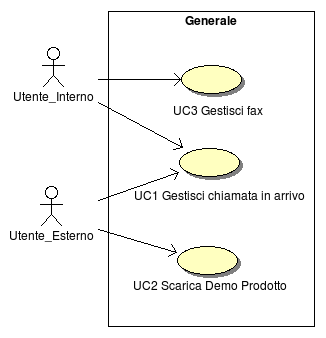
\includegraphics[scale=0.8]{./images/UC0_Generale.png}
\caption{UC0 - Generico}
\label{UC0}
\end{figure}

\newpage
\section{Formazione e Studio di fattibilit\` a}
La prima e consistente parte dello stage \`e iniziata con una breve fase di formazione guidata per prendere conoscenza del sistema informativo in uso e dei fondamentali processi aziendali. In particolare \'e stato messo l'accento sulle attivit\`a degli operatori commerciali, mostrandomi le varie fasi del loro lavoro, dall'acquisizione di un potenziale cliente fino alla sperabile vendita di uno o pi\'u prodotti, con tutti i passaggi intermedi. \\
Questo studio \`e stato eseguito con lo scopo di raccogliere pi\`u informazioni possibili per poter ideare un sistema che fosse il pi\`u possibile vicino ai bisogni dell'azienda con un occhio di riguardo verso modificabilit\'a e manutenibilit\'a, cosicch\'e chi dovr\`a successivamente correggere o estendere il modulo sviluppato si trovi nelle condizioni ideali per farlo. \\
Questa prima parte di formazione dunque ha permesso una comprensione del lavoro che si sarebbe dovuto andare a realizzare. Durante tali incontri c'\`e stata la possibilit\`a di dialogare con i rappresentanti delle aree di interesse dell'azienda, cos\`i da poter raccogliere informazioni, suggerimenti, richieste e lamentele riguardanti ogni aspetto che il sistema informativo avrebbe dovuto coprire. \\
L'esperienza accumulata durante questa fase ha portato ad una visione di insieme del progetto, che verr\`a rappresentata con la realizzazione di documenti che rappresentaranno quanto visto, eliminando le informazioni sovrabbondanti non riguardanti le fasi preliminari dello sviluppo. Un notevole supporto all'apprendimento della logica del sistema \`e venuto dalla gentile concessione dell'azienda, che ha permesso di effettuare una copia completa di tutti i codici sorgenti delle pagine PHP dell'applicazione, comprese anche alcune pagine del sito internet, in particolare quelle riguardanti i vari prodotti e il loro download, l'accesso in sola lettura al database (per non rischiare di comprometterne i dati) su cui tale applicazione si appoggia, e tutto il necessario per l'interfacciamento con il server Voispeed, per poter fare le dovute prove. \\
Il modulo assegnato, come tutti quelli previsti, doveva basarsi su un nuovo database sviluppato da due stagisti lo scorso anno, che effettuarono lo studio approfondito del vecchio sistema informativo ragionando sulla possibilit\`a di ristrutturazione del vecchio impianto, giungendo per\`o alla conclusione che l'unica alternativa percorribile era il completo rifacimento del tutto, per garantire maggiore flessibilit\`a. \\
La scelta di riscrivere il sistema ex novo comunque non avrebbe precluso la possibilit\`a di riutilizzare le porzioni di codice meglio realizzate: in particolare erano presenti numerose funzioni di recente implementazione che presentavano una buona qualit\`a del codice. Tali funzioni eseguivano operazioni complesse e meccaniche come la generazione delle fatture aderendo a strette regole di impaginazione o l'interfaccia del sistema con altri sistemi esterni che hanno necessit\`a di prelevare dati dal database. \\
Riutilizzando parte del codice preesistente e adattandolo al nuovo sistema sarebbe stato possibile  ridurre il tempo richiesto dalla noiosa implementazione di parti di poco interesse  e concentrarsi sulla progettazione delle nuove funzionalit\`a.

\section{Modulo VoIP e Fax}
Lo scopo principale del modulo VoIP e Fax \`e di permettere l'interazione dell'utente aziendale con il sistema informativo per gestire tutte le operazioni effettuate di prassi durante il proprio lavoro di rapporto e comunicazione con il cliente. Non richiede particolari funzionalit\`a complesse, se non una semplice visualizzazione comoda e intuitiva dei dati del cliente chiamante/chiamato per velocizzare tutte le operazioni da eseguire per un operatore commerciale. \\
Inizialmente con il committente si \`e discusso sulla possibilit\'a di adozione di un nuovo software PBX, analizzando in particolare le soluzioni open source basate sulla piattaforma Asterisk, molto flessibili ed economiche. Nonostante le funzionalit\'a aggiuntive e le promesse di risparmio, una scelta cos\'i forte sarebbe stata molto complicata da effettuare, in quanto i benefici sarebbero stati minimi se confrontati con gli svantaggi che sarebbero sopravvenuti, in particolare per gli operatori che avrebbero dovuto cambiare repentinamente le loro abitudini. \\
Siamo quindi giunti alla conclusione che fosse meglio studiare pi\'u a fondo le possibilit\'a proposte da Voispeed, che sono risultate sufficienti per ottenere i risultati prefissati. Nella fase di analisi dei requisiti ho potuto accedere al gestionale in uso presso la ditta, in aggiunta alla possibilit\`a di collegarmi al centralino VoIP, tramite i quali ho potuto analizzare quali dati avessero bisogno di essere gestiti dal modulo in procinto di essere sviluppato. \\
Inoltre tramite alcune interviste con alcuni dipendenti ho constatato di quali strumenti avessero bisogno per migliorare l'efficienza nel loro lavoro. Ed \`e proprio da queste interviste che sono emersi i requisiti principali di questo modulo, in quanto l'interazione dell'applicativo VOIce Client doveva essere plasmata secondo le necessit\`a di questi utenti. In seguito andr\`o ad analizzare le 3 sezioni in cui \'e suddiviso il modulo.

\newpage
\subsection{Integrazione Centralino VoIP}
\begin{figure}[!ht]
\centering
 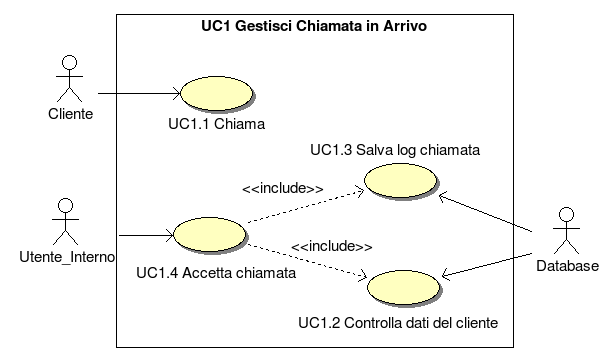
\includegraphics[scale=0.8]{./images/UC1_chiamata.png}
\caption{UC1 - Chiamata in arrivo}
\end{figure}

\noindent
Le azioni della prima delle sezioni trattate sopra descritte servono ad illustrare i processi che avvengono al seguito dell'arrivo di una telefonata da parte di un cliente che intenda parlare con il reparto commerciale dell'azienda o con l'assistenza tecnica. \\
In precedenza, per qualsiasi utente, l'unica informazione reperibile in questa fase era l'identit\`a del cliente/target chiamante, nel caso questo fosse registrato nel database aziendale, trovata utilizzando come parametro ovviamente il numero di telefono del chiamante. Dalle interviste effettuate, \`e emerso un bisogno generale di snellire tutte le operazioni che un commerciale era portato ad eseguire una volta ricevuta una telefonata, che principalmente erano raccogliere i dati del cliente chiamante dal sistema informativo tramite ricerca del nominativo, atto che portava per\'o ad uno spreco di tempo all'inizio della telefonata che in qualche caso poteva infastidire il cliente. \\
La necessit\'a primaria diventava quindi quella di poter ottenere pi\'u informazioni possibili all'arrivo di una chiamata, e di poter accedere immediatamente alla scheda del cliente con tutti i dati inseriti nel database. Inoltre altro bisogno indispensabile risultava l'automatizzazione della procedura di inoltro di una telefonata al commerciale tutelante del cliente chiamante, cosa che avveniva in modo del tutto privo di regole con situazioni paradossali all'interno degli uffici, come richieste a voce ai vicini di scrivania per stabilire a chi spettasse la telefonata.
\subsection{Invio Fax}
Il client VOIce integra una funzionalit\`a di invio fax, consentita per\'o solamente ad alcuni utenti abilitati all'invio. Necessit\`a degli utenti \'e di poter visualizzare l'elenco dei fax da loro inviati tramite un'apposita schermata del sistema informativo, in modo da avere a disposizione uno storico delle loro operazioni di invio.
\subsection{Ricezione Fax}
L'amministratore del sistema o chi abbia i permessi adeguati devono poter consultare i fax arrivati in azienda tramite apposita pagina del sistema informativo, e poter assegnarli al cliente corretto registrato nel database, non senza qualche nota a margine in caso di necessit\`a. Se il fax arrivato riguarda un particolare commerciale, questo deve poter essere informato tramite un'apposita funzione, in modo che questi possa leggerlo a sua volta.
\subsection{Use Cases}
\subsection*{UC1.1 Chiama}
\subsubsection*{Attori coinvolti} Cliente esterno, Server Voispeed.
\subsubsection*{Scopo e descrizione sintetica}
Il cliente telefona alla ditta, che gestisce la telefonata tramite il software VoIP.
\subsubsection*{Flusso di eventi}
\begin{enumerate}
\item Il cliente telefona all'azienda.
\item Il centralino VoIP riceve la telefonata e si prepara ad inoltrarla.
\end{enumerate}
\subsubsection*{Precondizioni}  Il centralino \` e in attesa di una telefonata esterna.
\subsubsection*{Postcondizioni} Il centralino ha risposto e attende di sapere dal cliente il tipo di operatore con cui questi vuole parlare.

\subsection*{UC1.2 Controllo del tipo di chiamata}
\subsubsection*{Attori coinvolti} Server Voispeed.
\subsubsection*{Scopo e descrizione sintetica}
Il centralino VoIP elabora la richiesta dell'utente impostando il reparto da contattare indicatogli dal cliente (commerciale, assistenza, amministrazione).
\subsubsection*{Flusso di eventi}
\begin{enumerate}
\item Il centralino ha ricevuto la telefonata.
\item Il centralino imposta il reparto al quale passare la telefonata.
\end{enumerate}
\subsubsection*{Precondizioni} Il centralino \` e pronto a selezionare il reparto da passare al cliente.
\subsubsection*{Postcondizioni} Il centralino ha impostato il reparto desiderato dal cliente chiamante.

\subsection*{UC1.3 Inoltra ad un utente del gruppo corretto}
\subsubsection*{Attori coinvolti} Server Voispeed, utente interno.
\subsubsection*{Scopo e descrizione sintetica}
Il centralino VoIP  inoltra la chiamata al reparto indicatogli dal cliente (commerciale, assistenza, amministrazione).
\subsubsection*{Flusso di eventi}
\begin{enumerate}
\item Il centralino verifica a che reparto passare la telefonata.
\item Il centralino inoltra la chiamata all'utente interno corretto.
\end{enumerate}
\subsubsection*{Precondizioni} Il centralino \` e pronto ad inoltrare la telefonata all'utente interno corretto.
\subsubsection*{Postcondizioni} Il centralino ha inoltrato correttamente la chiamata.

\subsection*{UC1.4 Controlla dati del cliente chiamante}
\subsubsection*{Attori coinvolti} Server Voispeed, Database.
\subsubsection*{Scopo e descrizione sintetica}
Nel caso di telefonata commerciale, il client Voispeed dell'utente a cui viene inoltrata la chiamata raccoglie i dati del cliente chiamante (tramite il numero di telefono e utilizzando il database) indicando, se presenti, le indicazioni sul commerciale che ha in tutela il dato cliente, seguendo le regole del regolamento interno dell'azienda.
\subsubsection*{Flusso di eventi}
\begin{enumerate}
\item Il client Voispeed dell'operatore controlla se il cliente chiamante \` e gi\` a tutelato da un commerciale per decidere a chi inoltrare la chiamata.
\end{enumerate}
\subsubsection*{Precondizioni} Il client \`e pronto a controllare quale operatore commerciale ha sotto tutela il cliente chiamante.
\subsubsection*{Postcondizioni} Il client ha controllato i dati del cliente, se esistente, e indica all'operatore chi, se presente, tutela il cliente che sta chiamando.

\subsection*{UC1.5 Salva il log della chiamata}
\subsubsection*{Attori coinvolti} Server Voispeed, Database.
\subsubsection*{Scopo e descrizione sintetica}
Il centralino VoIP salva nel database una traccia della telefonata avvenuta.
\subsubsection*{Flusso di eventi}
\begin{enumerate}
\item Il centralino raccoglie i dati della telefonata.
\item Il centralino scrive nel database tali dati.
\end{enumerate}
\subsubsection*{Precondizioni} Il centralino \`e pronto a registrare i dati della telefonata.
\subsubsection*{Postcondizioni} Il centralino ha registrato nel database i dati della telefonata avvenuta.

\newpage
\subsection{Requisiti}
\underline{\textbf{Funzionali}}
\begin{itemize}
\item Il sistema deve fornire all'utente del centralino che risponde alla chiamata tutti i dati utili riguardanti il cliente atti a snellire le operazioni da svolgere nell'arco della chiamata.
\item Il sistema deve permettere all'utente di utilizzare delle scorciatoie per l'accesso alle parti fondamentali del sistema operativo tramite un solo click del mouse.
\item Il sistema deve fornire tutte le funzioni per il trasferimento di chiamata dall'operatore commerciale che riceve la telefonata a quello che detiene la tutela del cliente chiamante.
\item Per gli operatori del Servizio Assistenza, il sistema deve fornire all'arrivo della chiamata tutti i dati riguardanti i software posseduti dal cliente chiamante e la loro copertura assistenziale.
\item Il sistema deve registrare i dati principali di una telefonata avvenuta come durata, numeri di telefono, data e ora di inizio e di fine. 
\item Il sistema deve permettere la consultazioni di tali tabulati, fornendo dei filtri per data e per utente interno. 
\item Il sistema deve permettere l'inserimento di un contatto telefonico solo se la telefonata relativa \'e effettivamente avvenuta.
\item Il sistema deve consentire ad un utente, che ha la possibilit\'a di inviare un fax, di visionarne l'elenco totale, tramite un \hyperlink{report}{\underline{report}} con gli appositi filtri applicati.
\item Il sistema deve permettere ad un amministratore di visualizzare i dati dei fax in arrivo e di poterli collegare al cliente corretto, con le dovute annotazioni opzionali. 
\item Un amministratore deve poter inoltrare un fax ricevuto all'operatore che sta seguendo la trattativa con quel cliente.
\item Il sistema deve fornire la possibilit\`a di visualizzare l'immagine del fax desiderato tramite la pressione di un unico pulsante.
\end{itemize}

\underline{\textbf{Di Qualit\`a}}
\begin{itemize}
\item Il codice scritto deve seguire le linee guida stabilite dagli stessi creatori di CodeIgniter \cite{cistyle}.
\item Il codice scritto deve basarsi sul pattern MVC.
\item Il codice xHTML e \hyperlink{css}{\underline{CSS}} devono essere validati dagli strumenti forniti dal \hyperlink{w3c}{\underline{W3C}} \cite{due}.
\item Il sistema deve garantire agli utilizzatori delle prestazioni accettabili.
\end{itemize}

\underline{\textbf{Di Interfacciamento}}
\begin{itemize}
	  \item Utilizzo del DBMS MySQL.
	  \item Il codice usato per la realizzazione delle classi deve essere il PHP.			
	  \item Utilizzo del framework CodeIgniter.
	  \item Utilizzo del web server Apache.
	  \item Utilizzo del software Voispeed per la gestione delle telefonate.
	  \item Il sistema informativo deve poter essere utilizzato con tutti i browser in circolazione attualmente.
	  \item Il sistema deve essere facile da utilizzare: tutte le funzionalit\`a devono essere disponibili all’utente, attraverso una comoda interfaccia grafica (pulsanti, caselle per l’input degli utenti, combobox, checkbox, ecc).
	  \item Il sistema informativo deve permettere all’utente di visualizzare in maniera facile veloce i dati di maggior interesse, mettendo a disposizione filtri e viste di vario genere, come i report dei fax e del registro delle chiamate.
\end{itemize}

\newpage
\section{Modulo Richieste}
Il secondo modulo raggiunge un livello di complessit\`a pi\'u elevato, a causa delle numerose variabili che entrano in contatto tra di loro. L'obiettivo in questo caso era quello di spostare la gestione delle richieste provenienti dal sito dell'azienda da GetResponse, un software di email marketing basato sul web che offre funzionalit\`a di spedizione di newsletters e di risposta automatica, al nuovo sistema informativo, per tenere traccia di tutte le operazioni svolte dai potenziali clienti interessati alle versioni dimostrative dei software sviluppati dall'azienda. 

\subsection{Gestione delle richieste}
\begin{figure}[!ht]
\centering
 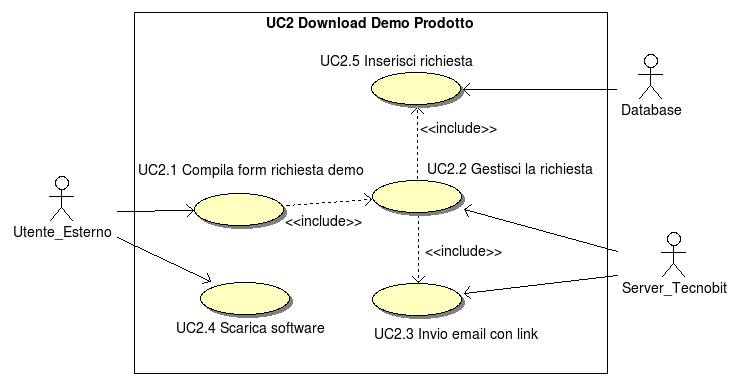
\includegraphics[scale=0.7]{./images/UC2_download.png}
\caption{UC2 - Download Versione Dimostrativa}
\end{figure}

\noindent
Requisito fondamentale era quindi quello di effettuare questa transizione in modo da automatizzare tutta la gestione delle richieste in arrivo utilizzando il sistema informativo aziendale, tracciando la fonte (che pu\`o essere un download di una versione dimostrativa dal sito dell'azienda, l'importazione da un database di contatti regolarmente acquistato, oppure la scansione di una apposita casella di posta elettronica dove vengono inoltrati i dati dei clienti italiani che hanno effettuato il download di una versione di prova del software Bricscad dal sito dello sviluppatore canadese), consentendo ad un amministratore di gestire l'elenco di queste richieste (acquisizione, assegnazione, cancellazione), e ad un utente commerciale di poterne acquisire una quantit\`a giornaliera limitata, seguendo un regolamento commerciale interno all'azienda.
\subsection{Use Cases}

\subsection*{UC 2.1 Compila Form Richiesta Demo}
\subsubsection*{Attori coinvolti} Utente Esterno, Server Tecnobit.
\subsubsection*{Scopo e descrizione sintetica}
L'utente esterno compila il form per scaricare un dimostrativo, richiedere un DVD o provare un programma nella sua versione online inserendo i propri dati personali specificando il prodotto selezionato.
\subsubsection*{Flusso di eventi}
\begin{enumerate}
\item Il cliente seleziona il prodotto del quale vuole richiedere una versione dimostrativa o altro.
\item Il cliente compila il form apposito per il download.
\end{enumerate}
\subsubsection*{Precondizioni} Il sistema ha caricato la pagina con il form per il download.
\subsubsection*{Postcondizioni} L'utente esterno ha compilato il form e ha inviato la richiesta al server.

\subsection*{UC 2.2 Gestisci la richiesta}
\subsubsection*{Attori coinvolti} Utente Esterno, Server Tecnobit.
\subsubsection*{Scopo e descrizione sintetica}
Il sistema elabora la richiesta effettuata dall'utente esterno.
\subsubsection*{Flusso di eventi}
\begin{enumerate}
\item Il cliente invia la richiesta cliccando sull'apposito tasto.
\item Il sistema elabora i dati inviati, controllando i dati del richiedente, nello specifico se \`e o no inserito nel database dell'azienda o se si tratta di un nuovo potenziale cliente.
\end{enumerate}
\subsubsection*{Precondizioni} L'utente ha compilato il form di richiesta.
\subsubsection*{Postcondizioni} Il sistema ha gestito la richiesta dell'utente.

\subsection*{UC 2.3 Invio e-mail con link}
\subsubsection*{Attori coinvolti} Utente Esterno, Server Tecnobit.
\subsubsection*{Scopo e descrizione sintetica}
Il sistema invia una mail all'utente con il link per procedere allo scaricamento della versione dimostrativa del prodotto.
\subsubsection*{Flusso di eventi}
\begin{enumerate}
\item Il sistema raccoglie i dati dell'utente, tra i quali l'indirizzo e-mail.
\item Il sistema invia la mail con il link per scaricare la versione dimostrativa del software scelto.
\end{enumerate}
\subsubsection*{Precondizioni} Il sistema ha ricevuto i dati dell'utente.
\subsubsection*{Postcondizioni} Il sistema ha inviato il link per lo scaricamento all'utente.

\subsection*{UC 2.4 Scarica Software}
\subsubsection*{Attori coinvolti} Utente Esterno, Server Tecnobit.
\subsubsection*{Scopo e descrizione sintetica}
L'utente scarica il software scelto dal link ricevuto per email.
\subsubsection*{Flusso di eventi}
\begin{enumerate}
\item L'utente riceve la mail.
\item L'utente scarica la demo tramite il link fornitogli.
\end{enumerate}
\subsubsection*{Precondizioni} L'utente attende la mail dal sistema.
\subsubsection*{Postcondizioni} L'utente ha scaricato la versione dimostrativa del software.

\subsection*{UC 2.5 Inserisci richiesta}
\subsubsection*{Attori coinvolti}  
Database, Server Tecnobit. 
\subsubsection*{Scopo e descrizione sintetica}
Nel database vengono inseriti i dati dell'utente che ha effettuato la richiesta di download. 
\subsubsection*{Flusso di eventi}
\begin{enumerate}
\item Il sistema raccoglie i dati dell'utente.
\item Viene creata una voce nel database che descrive l'utente e l'operazione da lui effettuata, per permettere agli 
operatori commerciali di contattarli successivamente.
\end{enumerate}
\subsubsection*{Precondizioni} Il sistema gestisce la richiesta.
\subsubsection*{Postcondizioni} Il sistema ha inserito la richiesta nel database in modo da poter contattare successivamente il cliente che l'ha effettuata.

\subsection{Requisiti}
\underline{\textbf{Funzionali}}
\begin{itemize}
  \item Il sistema deve consentire ad un cliente di scaricare la versione dimostrativa di un prodotto tramite una semplice pagina web.
  \item Il sistema deve inviare al cliente un' e-mail con all'interno il link per il download del demo del prodotto voluto. 
  \item Il sistema deve controllare i dati del cliente che effettua la richiesta, per verificare se questo \`e gi\`a inserito nel database aziendale.
  \item Nel caso il cliente sia gi\`a inserito, ed un commerciale lo abbia in tutela per il periodo corrente, il sistema deve inviare un messaggio a quest'ultimo per informarlo della richiesta avvenuta.
  \item Nel caso il cliente sia nuovo, ma proveniente da una provincia tutelata da un agente predefinito, quest'ultimo deve vedersi automaticamente assegnata la richiesta e inviato un messaggio per avvertirlo di questo, in modo che possa contattare il cliente il prima possibile.
  \item Nei casi in cui le richieste vengano assegnate automaticamente, un messaggio deve essere inviato anche agli amministratori di sezione, in modo che possano avere una traccia di ci\`o che avviene.
  \item Il sistema deve permettere all'amministratore di decidere quali richieste debbano essere visulizzabili da tutti i commerciali, e quali invece no.
  \item Il sistema deve consentire ad un commerciale di acquisire una richiesta pubblica per un numero di volte giornaliere stabilito a priori dall'amministratore.
  \item Il sistema deve permettere ad un amministratore di assegnare le richieste a piacere ad un commerciale, e avvisare ques'ultimo dell'assegnazione avvenuta tramite un messaggio.
  \item Il sistema deve provvedere a conteggiare la durata delle tutele di un cliente per un determinato utente, in modo da toglierle in caso di scadenza.
  \item Il sistema deve prevedere degli script pianificati che controllino tutte le tutele inserite in modo da eliminare quelle scadute.
\end{itemize}

\underline{\textbf{Di Qualit\`a}}\\
Valgono tutti i requisiti di questo tipo considerati per il modulo precedente.

\underline{\textbf{Di Interfacciamento}}\\
Valgono tutti i requisiti di questo tipo considerati per il modulo precedente.

\chapter{Svolgimento del Progetto: Sviluppo dei moduli}
\section{Il modello di sviluppo}
La necessit\`a di rendere il sistema estendibile e manutenibile ha richiesto l'adozione di un framework di sviluppo come CodeIgniter, il quale come detto si basa sul pattern architetturale MVC (Model-View-Controller) che ha come scopo quello di isolare la logica di business dell'applicazione dalla sua interfaccia con l'utente. Questa separazione rende molto pi\`u semplice la modifica della visualizzazione grafica o della logica sottostante senza dover adattare anche il resto dell'applicazione. In MVC, il model rappresenta l'informazione e le regole necessarie per manipolarla; la view corrisponde agli elementi dell'interfaccia utente che hanno il compito di presentare una certa visione dei dati; il controller gestisce gli eventi provenienti dall'utente ed eventualmente effettua opportune azioni sul model. \\
Nel caso di CodeIgniter, il controller si presenta come un una classe che contiene determinati metodi, ognuno rappresentante nella pratica una pagina. Questo controller nel suo costruttore si occupa di caricare tutti i models creati (loro stessi delle classi), tramite degli appositi costrutti del framework, per poi usarli nelle varie funzioni come qualsiasi istanze. Le views vengono caricate sempre tramite un funzione predefinita, con la possibilit\`a di passare loro i dati desiderati, siano essi le stesse istanze dei models, oppure altre variabili create nella funzione del controller.  \\
Tutta questa interazione porta al notevole vantaggio dell'indipendenza tra le parti: essendo infatti proprio il controller a gestire gli eventi, e i vari model a contenere ad esempio i metodi di recupero dati dal database, diventa possibile fare una modifica magari anche complessa senza influire mimimamente sul resto del sistema, arrivando ad avere una view che all'interno richiama gli stessi metodi, che in realt\`a possono essere stati completamente modificati dallo sviluppatore, magari per guadagnare in efficienza, o raccogliere una maggiore quantit\`a di dati da una chiamata al database.

\section{Progettazione e sviluppo}
Analizzati i requisiti dei moduli si \`e deciso di procedere quindi con la progettazione e lo sviluppo. In questo c'\`e stata la possibilit\`a di valutare la qualit\`a dell'analisi, gi\`a verificata con l'azienda, e di fornire un solido punto di partenza su cui ciascun modulo avrebbe potuto appoggiarsi in modo indipendente dagli altri che saranno sviluppati da altri stagisti. \\
Infatti, essendo l'obiettivo primario del rifacimento dell'intero sistema informativo la migliore efficienza, risulta conseguentemente anche la componente di maggior delicatezza ed interesse, che quindi necessita di pi\`u tempo per poter raggiungere una forma stabile. \\
Inoltre lavorare alla progettazione dei moduli seguendo l'analisi appena svolta, avrebbe permesso di valutare se i requisiti identificati fossero sufficientemente esaustivi o se invece alcuni aspetti erano stati omessi in sede di analisi.

\newpage
\subsection{Il Database}
Le prima azione da eseguire consisteva nella lieve ristrutturazione delle tabelle del database creato appositamente lo scorso anno. Essendo stata fatta una progettazione il pi\`u generale possibile, si \`e visto subito che alcune tabelle specifiche per i miei moduli erano assenti, come ad esempio \textit{clienti tel}, che associa ad un cliente pi\`u numeri di telefono, oppure \textit{utenti interni tutele}, che invece contiene i dati sulle tutele dei clienti da parte degli operatori commerciali. Un primo passo obbligato \`e stato quindi quello di integrare con le nuove tabelle il database, in modo da predisporlo allo sviluppo.

\begin{figure}[!ht]
\centering
  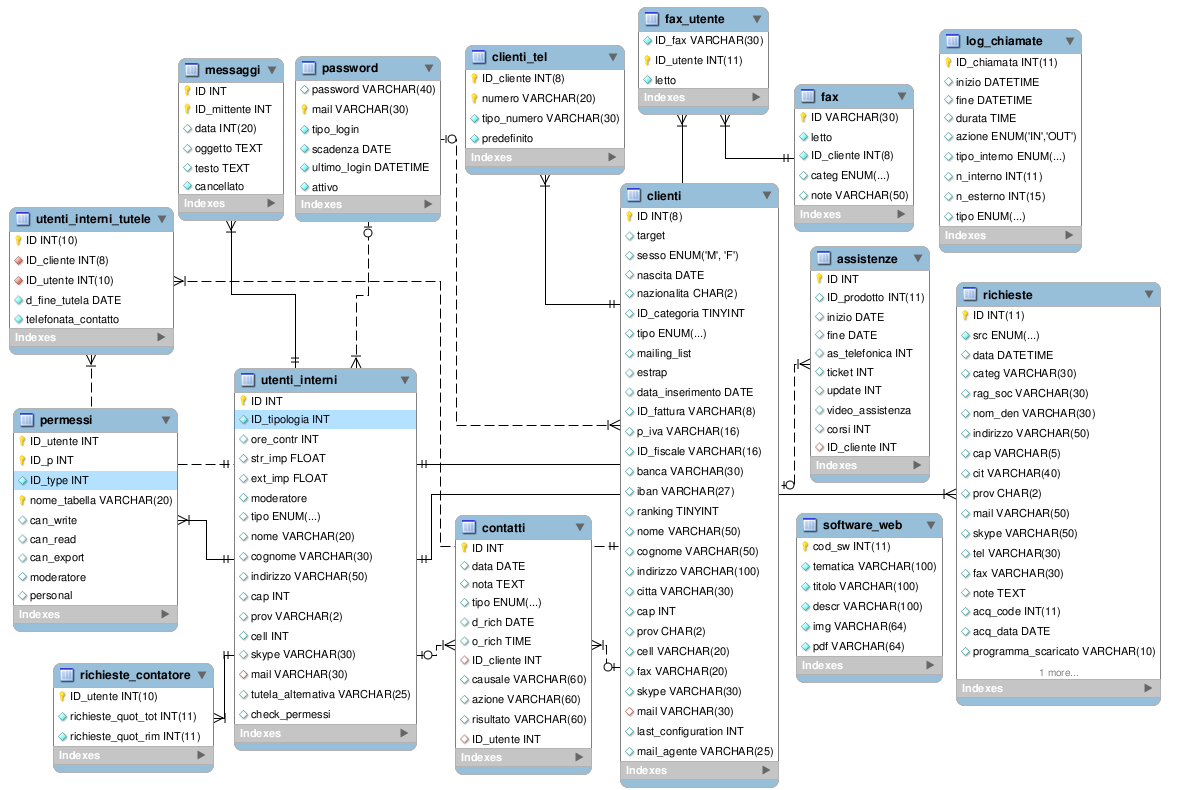
\includegraphics[scale=0.5]{./images/database.png}
\caption{Diagramma EER del database}
\label{EER}
\end{figure}

\noindent
Per rappresentare il \"{}frammento\"{} di database impiegato per i moduli, \`e stato usato un diagramma EER, ottenuto mediante il software gratuito MySQL Workbench. Il nuovo database come citato in precedenza era gi\`a pronto all'uso, ma molto generico e incompleto, per cui \`e stata necessaria una valutazione approfondita su quali carenze esso presentava, in modo da integrarlo con i dati mancanti ottenuti in seguito all'analisi. La figura \ref{EER} mostra tutte le tabelle utilizzate poi nello sviluppo di entrambi i moduli, comprese quelle accessorie, in modo da comprendere in modo ottimale il modo in cui si \`e lavorato successivamente nello sviluppo delle componenti, e il collegamento con il database sottostante. Le entit\`a che sono risultate evidenti come fulcro dei moduli sviluppati, attorno a cui ruotava la funzione delle altre entit\`a, sono state:
\begin{itemize}
  \item clienti
  \item contatti
  \item utenti interni
  \item fax
  \item richieste
  \item log chiamate
\end{itemize}

I collegamenti tra le varie entit\`a considerano i rapporti di integrit\`a referenziale tra i campi di tabelle diverse. Il vecchio database si basava su tabelle comunque dipendenti l'una dall'altra, ma senza alcun controllo, e questo negli anni ha portato alla creazione accidentale di molti doppioni che hanno solo aggiunto confusione al quadro gi\`a poco chiaro rappresentato dal database. In questo modo si \`e cercato di eliminare a monte tutte le possibili problematiche.
L'integrazione dei dati delle varie tabelle utilizzate \`e stata fatta tramite degli incontri con l'azienda in fase di analisi, in modo da evitare dei fastidiosi cambiamenti in fase di sviluppo che avrebbero creato notevoli problemi applicativi.

\newpage
\subsection{Il sistema informativo}
Basandosi quindi sul database appena descritto, tramite diagramma delle classi \hyperlink{uml}{\underline{UML}} viene descritta una prima struttura dei modulo da sviluppare, con le dipendenze esistenti derivanti dalla progettazione effettuata e dal pattern MVC utilizzato.

\subsubsection{VoIP}
\begin{figure}[!ht]
\centering
  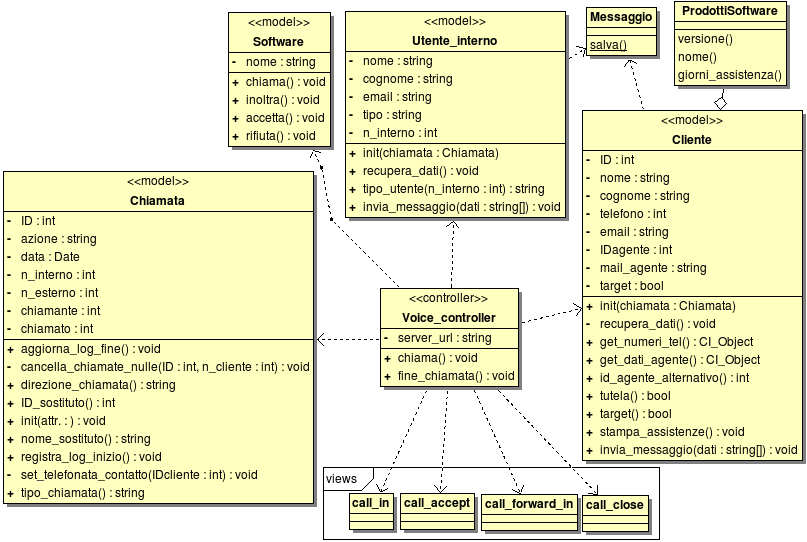
\includegraphics[scale=0.7]{./images/VoIPMVC.png}
\caption{Diagramma delle classi del modulo VoIP}
\label{voip}
\end{figure}

\noindent
Innanzitutto, dalla figura \ref{voip} si pu\`o notare come il fulcro del primo modulo sia sicuramente la \textit{Chiamata}, modello che contiene tutte le operazioni riguardanti una generica telefonata (in entrata o in uscita), come il salvataggio dei dati della chiamata in un apposito registro. Il controller ha il compito di raccogliere i dati di questa chiamata (per la maggior parte dall'integrazione con Voispeed) ed utilizzarli per chiamare le viste dedicate, a seconda dell'evento verificatosi(arrivo di una chiamata, oppure terminazione della stessa). Le classi \textit{Cliente} ed \textit{Utente Interno}, allo stesso modo, vengono istanziate dal controller ad ogni chiamata, e contengono i dati principali dell'utente interno e del cliente coinvolti nella telefonata, raccogliendone i dettagli dal database, come ad esempio il nome del proprio sostituto nel caso di un operatore commerciale, oppure le informazioni sulla tutela di un cliente e i prodotti per cui quest'ultimo abbia assistenza tecnica garantita. \textit{SoftwareProdotto} si occupa proprio della raccolta di questi dettagli, sfruttando le funzioni sviluppate da un'altro stagista, a cui era stato assegnato il modulo sulla gestione di un sistema per il supporto tecnico online. In particolare, l'istanza di tale classe permette di accedere ai dati di un cliente riguardanti prodotti ancora in assistenza, come nome, versione e giorni di assistenza mancanti, in modo da velocizzare le operazioni svolte dai tecnici, che all'arrivo di una chiamata riescono a conoscere in anticipo il contesto sul quale essa si baser\`a, conoscendo i prodotti posseduti dal cliente. 
La classe \textit{Software} cerca di astrarre le operazioni svolte dal client VoIP in modo da permettere una futura adozione, rapida e  indolore, di un nuovo software di questo tipo, raggruppando in metodi le normali azioni come l'accettazione, l'inoltro o il rifiuto di una chiamata. Questo comunque gi\`a dalle prime considerazioni fatte era apparso di difficile attuazione, a causa soprattutto della diversit\`a tra le API dei software, che nella maggior parte dei casi offrono funzionalit\`a magari simili tra loro ma implementate in modo molto diverso. 
La parte riguardante il registro delle chiamate non verr\`a illustrata con un diagramma, in quanto troppo semplicistica visto che le operazioni contenute nel modello riguardano solamente la visualizzazione di un report con lista delle telefonate avvenute tra un utente e i clienti nel tempo.
Segue ora una descrizione dei metodi pi\`u interessanti riguardanti il model implementato.
Per la chiamata:
\begin{description}
\item[- init] fa da \"{}costruttore\"{} per il modello Chiamata, inizializzando tutti gli attributi;
\item[- registra\_{}log\_{}inizio] crea un record nella tabella \textit{log\_{}chiamate} con i dati fondamentali della telefonata;
\item[- aggiorna\_{}log\_{}fine] aggiorna il record creato dal metodo precedente con i dati ottenuti alla terminazione della chiamata, in particolare la sua durata;
\item[- set\_{}telefonata\_{}contatto] attiva un flag che permetter\`a all'utente di aggiungere un contatto con il cliente segnandolo come \"{}telefonico\"{}, cosa che non pu\`o avvenire senza una telefonata;
\item[- tipo\_{}chiamata] ritorna il tipo di telefonata (assistenza tecnica, commerciale, ecc.);
\item[- cancella\_{}chiamate\_{}nulle] funzione di utilit\`a che cancella le chiamate registrate in modo incompleto presenti nel registro.
 \end{description}

per il cliente:
\begin{description}
\item[- init] inizializza, come nel modello precedente, il modello Cliente, utilizzando i dati della chiamata;
\item[- stampa\_{}assistenze] viene richiamato nel caso di una chiamata di assistenza tecnica, per stampare la tabella dei prodotti in assistenza per un dato cliente;
\item[- get\_{}numeri\_{}tel] ottiene i dati del cliente chiamante confrontando il suo numero con tutti i numeri di telefono memorizzati nel database;
 \end{description}

\newpage
\subsubsection{Fax}
\begin{figure}[!ht]
\centering
  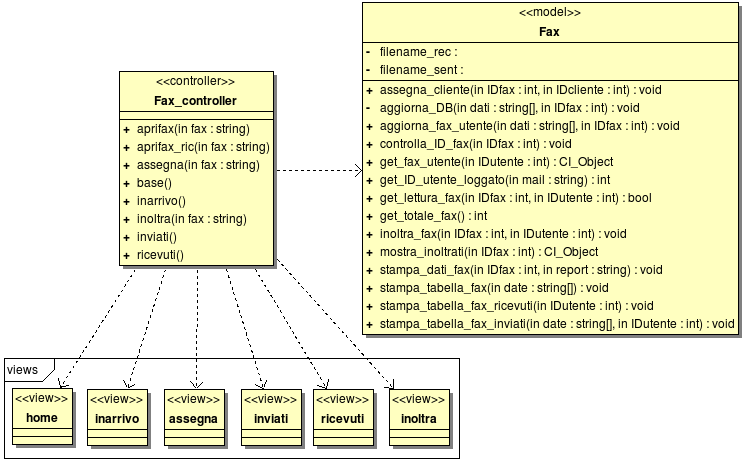
\includegraphics[scale=0.8]{./images/FaxMVC.png}
\caption{Diagramma delle classi della gestione Fax}
\label{fax}
\end{figure}

\noindent
La figura \ref{fax} illustra come il sistema gestisce tutte le operazioni effettuate sui fax. Il modello contiene i riferimenti ai due file di testo che Voispeed utilizza per tenere traccia dei fax inviati e ricevuti dal server, con la struttura di un file csv, e tutte le varie funzioni di utilit\`a per la loro gestione e visualizzazione nei report da costruire, come ad esempio il salvataggio di alcune note riguardanti i fax, oppure l'inoltro di uno di essi a un utente che possa esserne interessato.
A seguire, sono elencati i metodi pi\`u importanti nei modelli progettati.
\begin{description}
\item[- assegna\_cliente] consente di collegare un fax ad un cliente, per identificarne meglio la provenienza;
\item[- aggiorna\_DB] controlla la presenza dei dati di un fax nel database, e in caso contrario lo inserisce. E\` un metodo d'utilit\`a chiamato in determinate occasioni, per mantenere aggiornata la base dati;
\item[- inoltra\_fax] consente di collegare un fax ad un utente interno che pu\`o esserne eventualmente interessato, in modo che quest'ultimo possa consultarlo;
\item[- stampa\_dati\_fax] stampa i dati di un singolo fax nella tabella;
\item[- stampa\_tabella\_fax] costruisce l'elenco dei fax nell'intervallo di tempo selezionato.
\end{description}

\newpage
\subsubsection{Richieste}
\begin{figure}[!ht]
\centering
  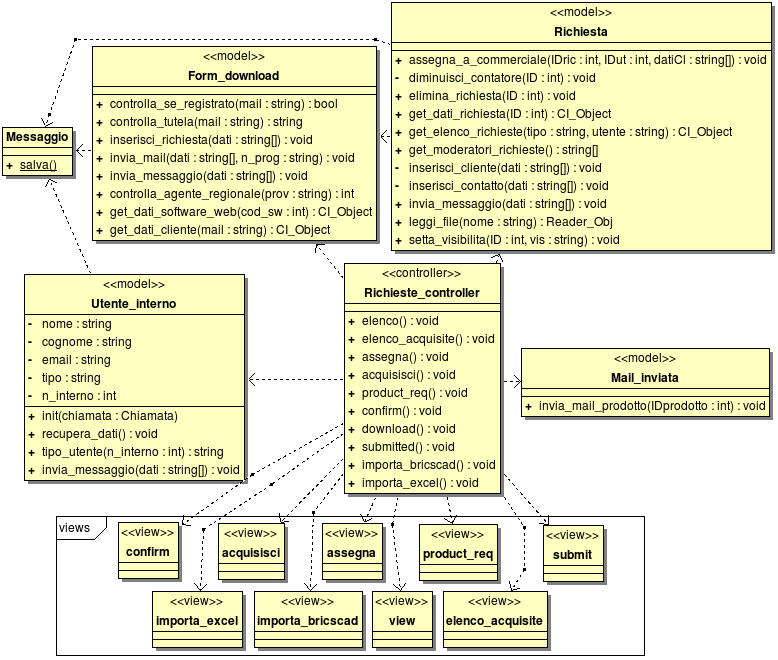
\includegraphics[scale=0.8]{./images/richiesteMVC.png}
\caption{Diagramma delle classi della gestione Richieste}
\label{richieste}
\end{figure}

\noindent
Andando ad analizzare il secondo e ultimo modulo, nella figura \ref{richieste}, si pu\`o vedere come la classe \textit{Richiesta} racchiude tutti i metodi per la gestione delle richieste memorizzate nel database, come la loro assegnazione, acquisizione e importazione da fonti diverse dal download diretto di un demo di un prodotto(in particolare da un foglio di calcolo o da una casella di posta ricevente mail propriamente formattate). Proprio per usufruire della prima possibilit\`a citata \`e presente la classe \textit{Form Download}, che controlla tutti i meccanismi riguardanti il salvataggio dei dati del cliente richiedente la versione dimostrativa, come ad esempio il controllo di tali dati per decidere come gestire la richiesta(come ad esempio nel caso la provincia di provenienza sia esclusiva di un agente aziendale), oppure l'invio dell' e-mail contenente i link(utilizzando i metodi resi disponibili dalla classe \textit{Mail inviata}), che contiene i metodi per inviare all'indirizzo fornito un'e-mail con le informazioni richieste a seconda del prodotto. Come nel caso di \textit{SoftwareProdotto}, la classe \textit{Messaggio} ed in particolare il metodo statico \textit{salva}() sono stati sviluppati da un altro stagista, in quanto entrambi i moduli specificati utilizzano in pi\`u occasioni i messaggi interni per la comunicazione tra sistema-utente, o anche utente-utente, per svariati bisogni, e appunto il metodo sopra citato permette di utilizzare l'infrastruttura della messaggistica interna per permettere al sistema di comunicare con gli utenti. Anche qui si pu\`o notare la presenza della classe \textit{Utente Interno}, come nel primo modulo, per tutte le operazioni e informazioni riguardanti l'utente collegato al sistema informativo, come ad esempio i permessi posseduti.
A seguire, sono elencati i metodi pi\`u importanti nei modelli progettati.
Per il form di download:

\begin{description}
\item[- controlla\_{}se\_{}registrato] confronta i dati inseriti dal cliente con il database per verificare un'eventuale presenza;
\item[- controlla\_{}agente\_{}regionale] controlla se la provincia inserita dal cliente \`e tutelata in esclusiva da un agente provinciale dell'azienda;
\item[- get\_{}dati\_{}software\_{}web] ricava i dati dei prodotti per i quali \`e possibile scaricare la versione dimostrativa;
\item[- controlla\_{}tutela] controlla se il cliente, gi\`a registrato, sia anche gi\`a tutelato da un operatore commerciale;
\item[- invia\_{}mail] invia l'e-mail corretta con i link per lo scaricamento della demo al cliente.
\end{description}
\noindent
Per le richieste:
\begin{description}
\item[- assegna\_{}a\_{}commerciale] si occupa di effettuare tutte le operazioni seguenti all'acquisizione di una richiesta, come la creazione di una nuova scheda cliente, e di un primo contatto che descrive quando questa \`e stata creata;
\item[- diminuisci\_{}contatore] diminuisce il contatore delle richieste giornaliere, fino a che questo \`e possibile;
\item[- get\_{}moderatori\_{}richieste] ottiene la lista degli amministratori della sezione richieste, in particolare per generare un messaggio ad inviare a questi per avvertirli di una richiesta acquisita automaticamente da un agente provinciale o da un operatore che possiede la tutela esclusiva su un cliente;
\item[- get\_{}elenco\_{}richieste] ricava la lista totale delle richieste, per fornirle ai vari elenchi.
\end{description}


%-----------------------------------------------------------------------
%-----------------------------------------------------------------------
%-----------------------------------------------------------------------
%-----------------------------------------------------------------------

\newpage
\section{Realizzazione}
Verranno illustrate ora le soluzioni adottate per lo sviluppo dei due moduli, associando alla descrizione delle scelte effettuate, citando metodi principali e procedure, alcune immagini per comprendere al meglio il contesto, compresi screenshot raccolti ad hoc per comprendere al meglio quanto descritto e frammenti di codice rappresentativo.
\subsection{Modulo VoIP e Fax}
\subsubsection{Gestione Chiamate}
Per la parte riguardante il VoIP, e quindi l'interazione con il sofware Voispeed, occorre una piccola introduzione riguardo al suo funzionamento. La figura \ref{integra} (presa direttamente dal manuale online del software, \cite{voispeed}), mostra quale sia l'interfaccia (in questo caso lato client, ma nel nostro caso regolata dal server) tramite la quale vengono gestiti gli eventi da integrare e il comando da dare alla loro esecuzione: \\

\begin{figure}[!ht]
\centering
  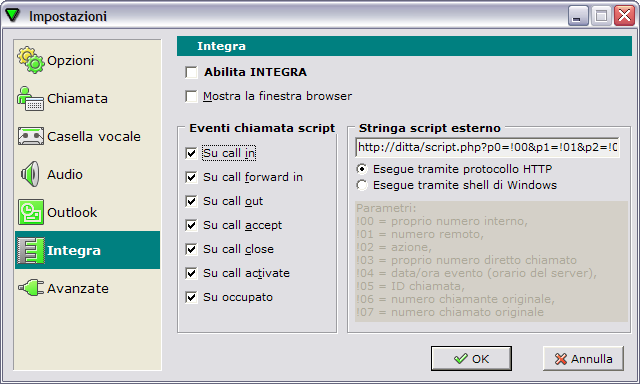
\includegraphics[scale=0.6]{./images/voispeedoptions.png}
\caption{Interfaccia Integra}
\label{integra}
\end{figure}

\noindent
Il client infatti permette di sfruttare delle pagine web opportunamente costruite, passando come parametri mediante il metodo GET dell'\hyperlink{html}{\underline{HTML}}, unica possibilit\`a offerta nonostante la nota fragilit\`a (l'utilizzo del metodo POST non \`e contemplato dal software), il quale \`e usato come mezzo per l'invio dei dati come parte di un \hyperlink{url}{\underline{URL}}. \\
Alla ricorrenza di un determinato evento riguardante la chiamata, \`e possibile collegare il VOIce client ad una pagina web e passare pi\`u dati contemporamente, tra i quali: 
\begin{itemize}
 \item !00 = proprio numero interno;
 \item !01 = numero remoto (chiamato o chiamante);
 \item !02 = azione (evento che ha attivato l'invocazione dello script e corrisponde a quelli che si possono selezionare);
 \item !05 = ID della chiamata (generato automaticamente dal Server e identifica in modo univoco la chiamata);
 \item !06 = numero chiamante originario (questo parametro indica il numero effettivo del chiamante);
 \item !07 = numero chiamato originale (questo parametro indica il numero effettivo chiamato dall'utente remoto).
\end{itemize}
\noindent
Utilizzando appunto questi parametri tramite il controller \textit{call} e la sua funzione interna \textit{chiama}(), alla quale vengono passati ad ogni evento prestabilito nella configurazione (nella fattispecie: CALL\_IN, CALL\_ACCEPT, CALL\_CLOSE e CALL FORWARD IN), \`e stato possibile richiamare le pagine corrette semplicemente tramite l'apposita istanza del browser Internet Explorer utilizzata dal client. \\
Ad esempio se arrivasse una chiamata dall'esterno dal numero 02675456 a cui rispondere per l'utente con ID=6, allora si avrebbe: !02=CALL\_IN, !06=02675456, e !07=6. Utilizzando queste funzionalit\`a, \`e stata associata una pagina da visualizzare per ogni evento sopra descritto, che appare all'utente una volta che tale evento si attiva. 

\newpage
Ad esempio, come mostrato nella figura \ref{chiamata_comm}, ad una chiamata in arrivo verr\`a visualizzata questa finestra all'operatore commerciale:

\begin{figure}[!ht]
\centering
  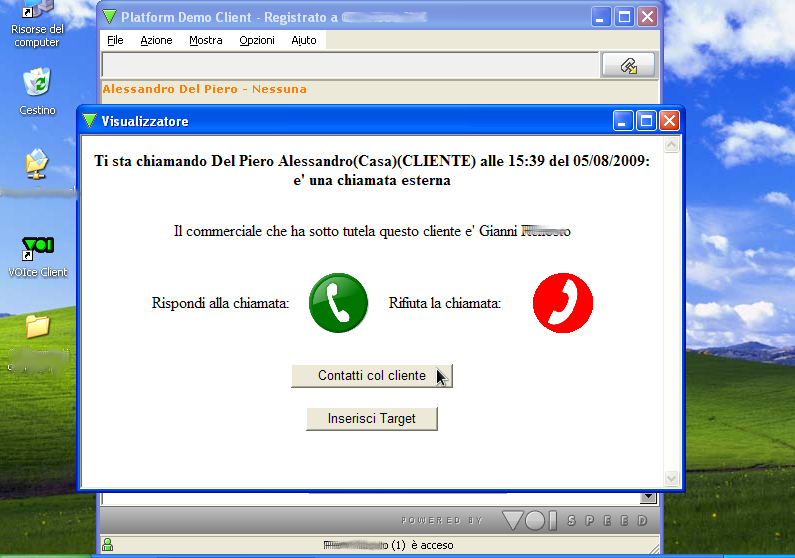
\includegraphics[scale=0.8]{./images/chiamata_commerciale.png}
\caption{Chiamata in arrivo a Commerciale}
\label{chiamata_comm}
\end{figure}

\noindent
Come si pu\`o vedere, il sistema informativo controlla nel database se il numero di telefono chiamante \`e collegato ad un cliente, fornendone i dati utili all'operatore a cui arriva la telefonata, nel caso siano presenti. In particolare, oltre al nome e la qualifica del cliente, viene mostrato anche il nome dell'operatore commerciale che, nel periodo corrente, detiene la tutela esclusiva sul cliente in questione. \\
Questa informazione \`e sicuramente la novit\`a principale che riguarda questa parte, in quanto in precedenza ad ogni telefonata si creava una certa confusione per trovare questo dato, dovendo effettuare ogni volta una ricerca manuale nel (lento) sistema informativo per trovare chi, se presente, avesse il diritto alla tutela, e girare a questa persona la telefonata. \\
Questo problema viene ora superato fornendo a chi risponde tutte le scorciatoie necessarie ad effettuare questa procedura in modo semi-automatico, guidando l'utente passo passo (tramite l'utilizzo di alcune funzionalit\`a del framework \hyperlink{javascript}{\underline{javascript}} jQuery \cite{jquery}. \\
Il diagramma della figura \ref{act_call} mostra quale sia il flusso della funzione \textit{chiama}() presente nel classe controller per la gestione delle chiamate. 

\begin{figure}[!ht]
\centering
  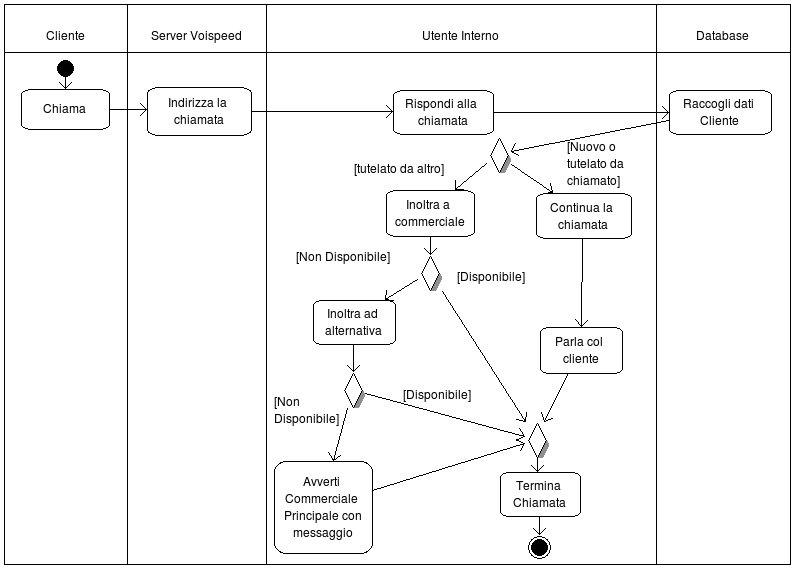
\includegraphics[scale=0.7]{./images/chiamataAct.png}
\caption{Diagramma di attivit\`a relativo alla funzione \textit{chiama}() del controller}
\label{act_call}
\end{figure}

\noindent
Questo flusso analizza quindi gli eventi successivi all'arrivo e accettazione di una chiamata da parte di un operatore commerciale, il quale riceve tramite l'interfaccia di VoICE Client tutte le informazioni necessarie sul cliente chiamante. L'utente viene immediatamente avvertito riguardo alla tutela di questo cliente, che pu\`o essere:
\begin{itemize}
 \item nuovo (e quindi con la possibilit\`a di trattare liberamente);
 \item presente nel database ma al momento fuori tutela (quindi si pu\`o procedere come sopra);
 \item gi\`a tutelato da un'altro operatore: il sistema fornisce l'identit\`a dell'agente corretto a cui inoltrare la chiamata.
\end{itemize}
\noindent
A questo punto, al seguito dell'accettazione della telefonata, all'utente vengono fornite una serie di funzionalit\`a atte a permettere l'inoltro della telefonata all'utente che possiede l'esclusiva sul cliente, tramite dei pulsanti presentati in modo molto semplicistico: nel caso questi sia occupato o assente, subito il sistema fornisce dinamicamente le opzioni per la chiamata di un sostituto, segnalato appunto se necessario. In caso nemmeno questo sia raggiungibile, l'utente riattiva la chiamata con il cliente, assicurandolo che verr\`a ricontattato a breve, e al termine della telefonata gli viene proposto un pulsante che invia un messaggio automatico (tramite il sistema di messaggistica interno) con gli estremi della chiamata al tutelante, informandolo di contattare al pi\`u presto il cliente. La figura \ref{forward_call} illustra appunto una fase di questo iter. 

\begin{figure}[!ht]
\centering
  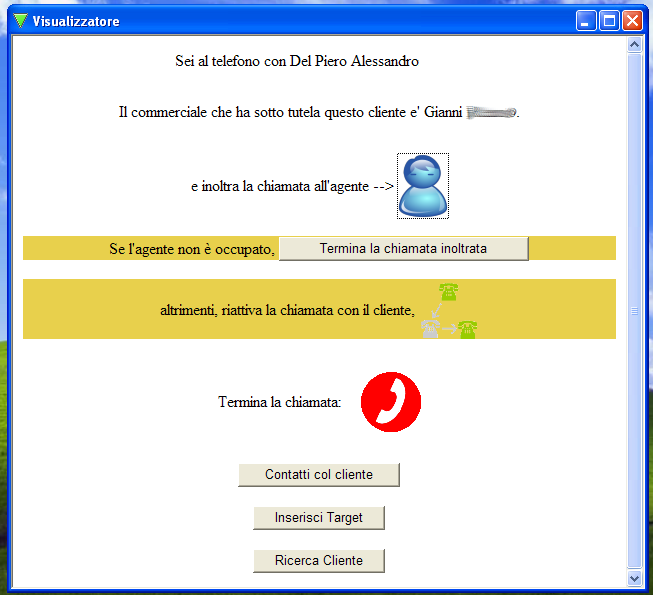
\includegraphics[scale=0.75]{./images/inoltroScreen.png}
\caption{Inoltro di una chiamata}
\label{forward_call}
\end{figure}

\noindent
Nella fattispecie, nell'istante rappresentato l'utente ha provato ad inoltrare la chiamata, e il sistema gli propone le varie possibilit\`a selezionabili. Il tutto \`e reso dinamico grazie all'utilizzo di jQuery, e in particolare i metodi \textit{slideDown}() e \textit{slideUp}() che offre, per far apparire e scomparire i pulsanti in sequenza. Qui di seguito ecco un esempio di codice utilizzato:


\begin{verbatim}
    $("#attesa").click(function () {
             $("#chiamaInoltro").slideUp("slow");
             $("#terminaNonOccupato").slideUp("slow");
             $("#riattiva").slideUp("slow");
             $("#riattivaSub").slideDown("slow");
    });
\end{verbatim}               

\noindent
che fa apparire e scomparire con un effetto di scorrimento i quattro elementi contenuti al click del mouse sull'elemento \"{}attesa\"{} (identificato dall'icona con i tre telefoni collegati di figura \ref{forward_call}). \\
\noindent
Nel caso invece della chiamata in arrivo per un tecnico dell'assistenza tecnica(figura \ref{technical_call}), il sistema elaborer\`a i dati derivanti dalla chiamata in modo da fornire questa volta le informazioni riguardanti i prodotti in assistenza al momento della chiamata, in forma tabellare. In questo modo il tecnico viene a conoscenza in anticipo dei prodotti posseduti dal cliente, riuscendo a velocizzare i tempi di risoluzione.

\begin{figure}[!ht]
\centering
  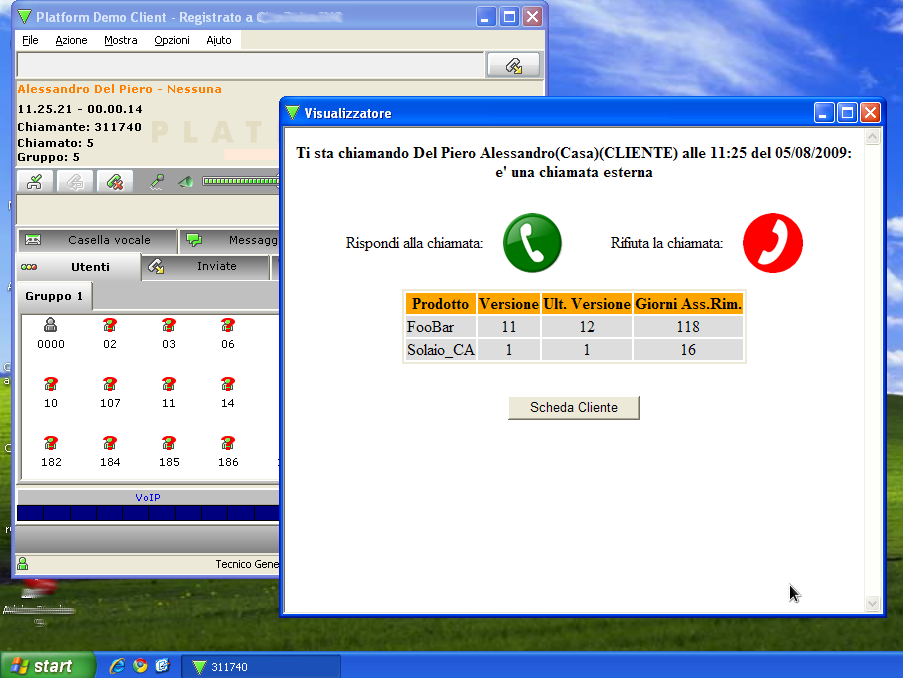
\includegraphics[scale=0.6]{./images/chiamata_assistenza.png}
\caption{Chiamata all'assistenza tecnica}
\label{technical_call}
\end{figure}

\newpage
\subsubsection{Gestione Fax}
Per la gestione dei fax in arrivo e inviati, si \`e dovuto analizzare il sistema di funzionamento di Voispeed Server, che salva in due file di testo contenuti nella cartella d'installazione i log riguardanti questi fax, rispettivamente \textit{RecvFax.txt} e \textit{SentFax.txt}. Entrambi sono strutturati come file *.csv, e rispettivamente con i dati posizionati negli esempi seguenti:
\begin{verbatim}
    20051019163859781,9,Ricezione completa,0424568458,0424123123,
    FAXREC2005101916374901501,Ditta International
\end{verbatim} 
per il primo, e cos\`i
\begin{verbatim}
    20060227131108607,12,Consegnato,nome.cognome,
    0801541111 - PINCO PALLINO,1,FAX20060227130823107
\end{verbatim} 
\noindent per il secondo.
Strutturalmente si presentano lievemente diversi, in quanto per i fax inviati non \`e contenuto il numero di invio, sostituito invece con il nome dell'utente registrato in Voispeed che ha inviato il fax. Il resto dei parametri \`e invece comune ad entrambi, come data e ora (precise al secondo), l'ID univoco del fax, il nome del cliente contattato se memorizzato nella rubrica del software, e lo stato del fax (ricevuto, consegnato, ecc.). \\
La creazione dei report nel sistema informativo quindi necessita strettamente della lettura da tali file, in quanto il server Voispeed aggiunge una nuova riga al log ad ogni operazione effettuata, rendendo necessaria una nuova lettura ad ogni accesso al report. Inoltre il committente desiderava poter collegare altre informazioni ad ogni fax, come ad esempio il cliente a cui associarlo, una categoria specifica e, nel caso servissero, delle note su qualche dettaglio. \\
Questo bisogno \`e sfociato nella scelta di effettuare una \"{}sincronizzazione\"{} tra database e tali file di log, in modo da mantenere nel primo i dati sopra citati, voluti dal cliente, e nel secondo leggere progressivamente le informazioni fornite da Voispeed. Questo \`e stato possibile grazie all'implementazione del metodo descritto in sede di progettazione \textit{aggiornaDB}(), che si occupa, ad ogni richiesta al server del report dei fax in arrivo, di verificare l'effettiva presenza nel database(confrontando l'ID univoco del fax), e in caso negativo inserire i dati mancanti. 

\newpage
\begin{figure}[!ht]
\centering
  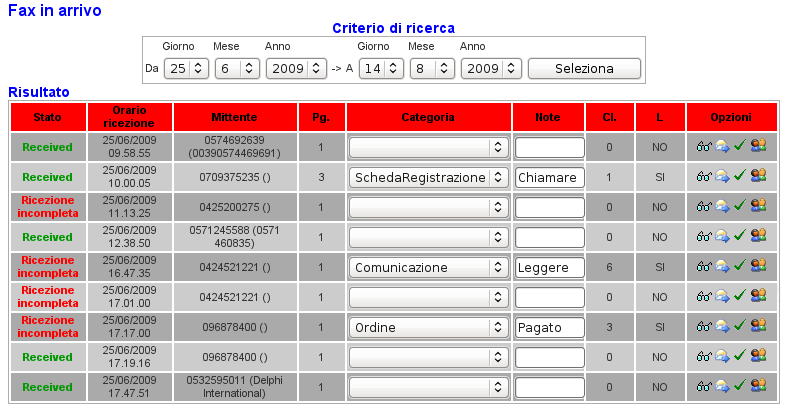
\includegraphics[scale=0.8]{./images/faxinarrivo.png}
\caption{Report dei fax in arrivo}
\label{fax_in_arrivo}
\end{figure}

\noindent
La figura \ref{fax_in_arrivo} mostra la soluzione grafica scelta per il report dei fax in arrivo. Questo \`e accessibile solamente agli utenti con i permessi appropriati, tra i quali sono presenti ovviamente gli amministratori, ma anche i dipendenti del reparto amministrativo. Una volta selezionato l'intervallo temporale entro il quale visionare l'elenco dei fax, per ognuno di questi il sistema offre la possibilit\`a, tramite i quattro pulsanti sulla destra, di:

\begin{itemize}
 \item visualizzarlo, caricando il file immagine in formato tiff corrispondente;
 \item inoltrarlo a un operatore commerciale che ne pu\`o essere interessato;
 \item salvarne i dati nel database (categoria, note);
 \item collegarlo ad un particolare cliente che pu\`o ad esempio averlo inviato.
\end{itemize}

Gli altri due report disponibili invece sono messi a disposizione degli utenti commerciali generici, che possono visualizzare i fax personali ricevuti (assegnati tramite l'inoltro citato prima nell'elenco), ed inviati (se ne hanno il permesso).
\newpage
Nella figura \ref{codice_fax} viene illustrata la porzione di codice php della funzione \textit{stampa\_{}tabella\_{}fax}() che illustra l'algoritmo per la scansione del file dei fax in arrivo:

\begin{figure}[!ht]
\centering
  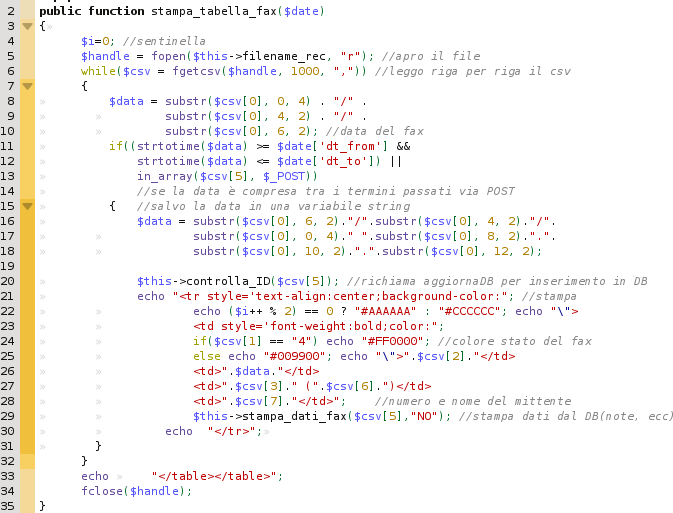
\includegraphics[scale=0.6]{./images/codicefax.png}
\caption{Frammento di codice per la lettura dei fax}
\label{codice_fax}
\end{figure}

\noindent
Come si pu\`o vedere, la funzione scansiona riga per riga il file tramite gli appositi metodi forniti dal linguaggio PHP, prendendo l'intervallo di tempo selezionato dall'utente come parametro in ingresso, e usandolo come discriminante per la stampa(riga 11): solo i fax ricevuti in tale intervallo verrano stampati a video nel report, con i loro dati fondamentali. Il metodo chiama poi \textit{stampa\_{}dati\_{}fax}(), che completa la riga della tabella con i dati raccolti dal database tramite l'ID del fax, contenuta chiaramente nella variabile \textit{csv[5]}(riga 29).

\newpage
\subsection{Modulo Richieste}

Il modulo riguardante le richieste invece si basa principalmente sul rapporto che intercorre tra il cliente (il pi\`u delle volte potenziale) che decide di scaricare la versione dimostrativa di un programma, e il sistema informativo che deve gestire tale richiesta il pi\`u efficientemente possibile.

\subsubsection{Visualizzazione Richieste}
\begin{figure}[!ht]
\centering
  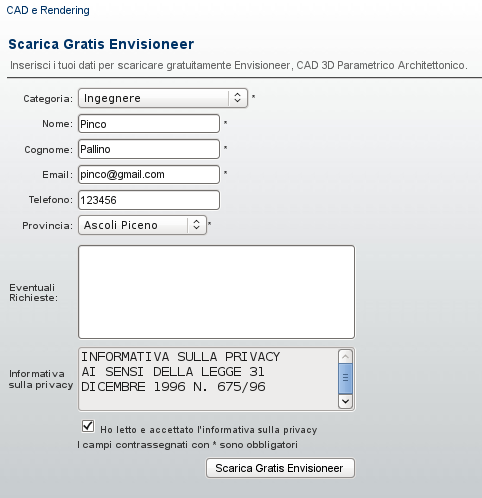
\includegraphics[scale=0.75]{./images/downloadScreen.png}
\caption{Form di download di una demo}
\label{form_download}
\end{figure}

\noindent
La figura \ref{form_download} mostra la form che appare al cliente nel momento successivo al click sul pulsante di download: una volta inseriti i dati (controllati dinamicamente sia tramite codice Javascript, sia lato server) e cliccato sul pulsante per lo scaricamento, il sistema invia un'e-mail con i link necessari allo scaricamento e utilizzo della versione dimostrativa del prodotto voluto.
L'invio della mail al cliente, attivit\`a svolta a prescindere dalle informazioni su quest'ultimo, avviene automaticamente dal server dell'azienda, sfruttando l'helper appositamente concepito dagli sviluppatori di CodeIgniter. La documentazione \`e estremamente chiara riguardo al suo utilizzo, ma nella figura \ref{mail_sending} viene illustrato quanto semplice sia inviare una mail utilizzando queste funzionalit\`a:


\begin{figure}[!ht]
\centering
  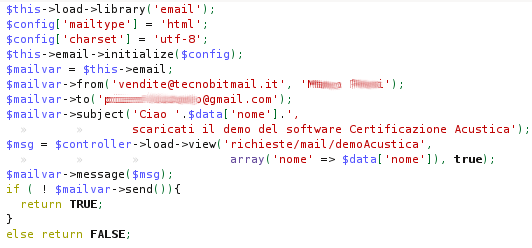
\includegraphics[scale=0.8]{./images/codiceinviomail.png}
\caption{Codice per l'invio di una mail al cliente}
\label{mail_sending}
\end{figure}

\noindent
Tramite la variabile \textit{\$mailvar}, chiaro riferimento all'helper, il sistema imposta i dati principali della mail da inviare (destinatario, mittente, oggetto) e carica il testo da una pagina HTML precedentemente preparata riferita al prodotto selezionato (la variabile \textit{\$msg}), e la manda al cliente, controllando inoltre se il tutto sia avvenuto correttamente. Ovviamente il \hyperlink{mail_server}{\underline{mail server}} deve essere configurato correttamente per l'invio.
\newpage


\begin{figure}[!ht]
\centering
  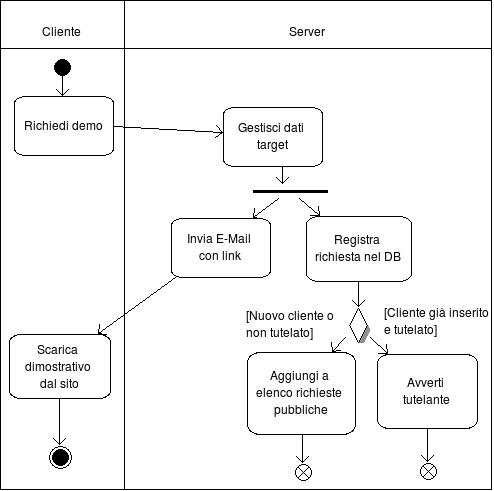
\includegraphics[scale=0.75]{./images/downloadAct.png}
\caption{Diagramma di attivit\`a per la procedura di download}
\label{download_act}
\end{figure}

\noindent
Il diagramma di figura \ref{download_act} mostra il flusso di azioni successive alla compilazione del form da parte del cliente. Una volta acquisiti i dati, il sistema compie parallelamente due azioni distinte, compiute nella funzione \textit{confirm}() del controller: da una parte si occupa di inviare l'e-mail con i link al richiedente; dall'altra confronta i dati presenti nel database, verifica le informazioni ricevute e:

\begin{itemize}
 \item nel caso sia gi\`a registrato e tutelato, invia un messaggio automatico all'operatore commerciale che detiene la tutela, informandolo circa l'azione compiuta dal cliente: sar\`a suo compito gestire i rapporti futuri, contattando l'interessato per cercare di vendere il programma in prova;
 \item nel caso sia registrato ma non tutelato, aggiunge la richiesta all'elenco delle richieste pubbliche: ogni commerciale da questo elenco pu\`o acquisire la richiesta voluta, con un limite giornaliero prefissato;
 \item nel caso sia un nuovo cliente, aggiunge sempre una nuova richiesta come nel caso precedente.
\end{itemize}
\noindent
Esiste un caso particolare riguardo alla tutela: infatti l'azienda contempla il ruolo di \"{}agente provinciale\"{}, il quale ha il completo controllo sulla clientela proveniente da una certa provincia. Ad esempio, al momento ne \`e presente uno per tutte le province della Sardegna, che quindi pu\`o liberamente trattare senza limite con i clienti di questa regione, senza alcun vincolo temporale.\\
Di questo filtro per provincia si occupa la funzione \textit{controlla\_{}agente\_{}regionale}(), che si occupa di inserire in automatico una scheda cliente ed avvisa, sempre tramite il sistema di messaggistica interno, l'agente designato, che viene invitato a contattare al pi\`u presto il cliente stesso.

\begin{figure}[!ht]
\centering
  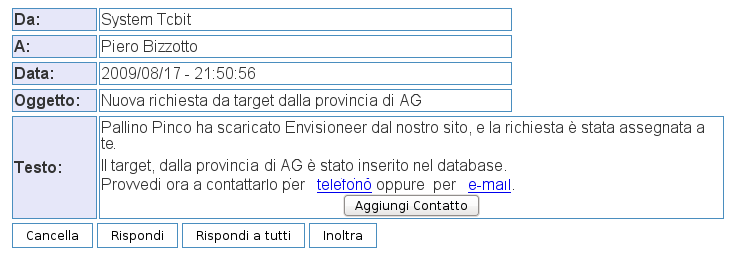
\includegraphics[scale=0.5]{./images/messaggioAgenteScreen.png}
\caption{Messaggio ad un agente provinciale}
\label{agent_message}
\end{figure}

\noindent
Il messaggio \`e simile a quello nella figura \ref{agent_message}, che una volta letto mostra alcune informazioni riguardo il cliente potenziale che ha effettuato il download della demo, comprese anche delle scorciatoie (numero di telefono ed e-mail) utili per un immediato contatto.
Nel caso il cliente sia gi\`a presente e tutelato da un operatore commerciale, il sistema invia un messaggio simile per informarlo del fatto, fornendo le stesse scorciatoie. 
Terminata la spiegazione riguardante i messaggi interni, l'analisi si sposta all'elenco delle richieste pubbliche, e in particolare nel caso dellle funzioni disponibili ad un amministratore della sezione.
\newpage

\begin{figure}[!ht]
\centering
  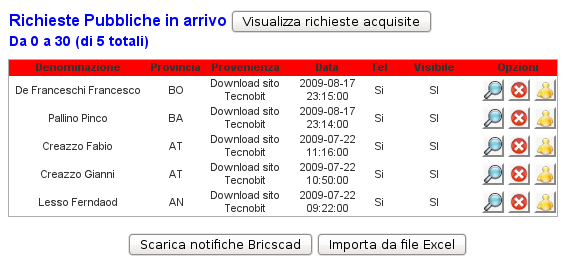
\includegraphics[scale=0.6]{./images/elencoRichiesteScreen.png}
\caption{Elenco di richieste in arrivo}
\label{elenco_richieste}
\end{figure}

\noindent
La figura \ref{elenco_richieste} mostra le informazioni fornite dal report per ogni richiesta in arrivo ancora libera, dal punto di vista di un amministratore. Questi, per ognuna, ha la possibilit\`a di acquisirla (come verr\`a spiegato in seguito), cancellarla oppure assegnarla ad un operatore commerciale qualsiasi, a sua discrezione. Inoltre pu\`o decidere di nascondere alcune richieste nel caso avesse bisogno di approfondire alcuni dettagli su un possibile cliente.
Un semplice utente, invece, all'apertura dell'elenco pubblico, pu\`o semplicemente decidere di acquisire alcune di queste richieste, rispettando il limite giornaliero a lui assegnato. 

\begin{figure}[!ht]
\centering
  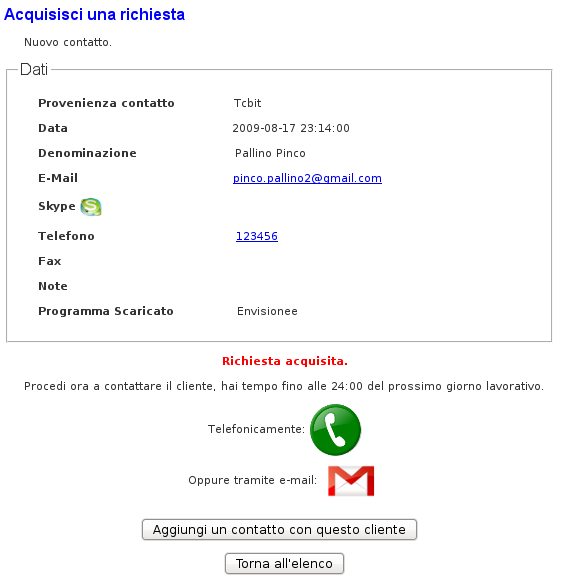
\includegraphics[scale=0.6]{./images/acquisisciScreen.png}
\caption{Acquisizione di una richiesta}
\label{acq_richieste}
\end{figure}

\noindent
\newpage
Questa acquisizione, mostrata nella figura \ref{acq_richieste} nella sua fase terminale, \`e fattibile con pochi clic da parte dell'utente commerciale. Una volta terminata, questi ha 24 ore (previste dal regolamento commerciale in vigore attualmente) per effettuare un primo contatto, e il sistema si occupa di inserire subito una scheda per il cliente. Se l'utente non effettua questo contatto, la richiesta torna automaticamente nell'elenco pubblico, pronta per essere raccolta da qualche altro utente interessato.


\newpage
\subsubsection{Importazione richieste}
Altra funzionalit\`a richiesta con una certa priorit\`a era sicuramente la possibilit\`a di importare elenchi di richieste da database esterni, la maggior parte acquistati come file excel oppure, sistema non meno importante, scansionando una casella e-mail opportunamente predisposta a ricevere messaggi strutturati allo stesso modo.
Il primo metodo \`e sicuramente di importanza capitale in quanto permette un'acquisizione immensa di potenziali clienti, e per questo \`e stata sviluppata appositamente una pagina, accessibile ai soli amministratori, tramite la quale importare tali file in modo da rendere semplice l'operazione. Per raggiungere questo risultato \`e risultata adatta la libreria PHP Excel Reader \cite{excel reader}, tanto facile da utilizzare quanto potente \cite{cinque}, capace di trasformare un file excel in una tabella HTML, e di leggerlo cella per cella.

\begin{figure}[!ht]
\centering
  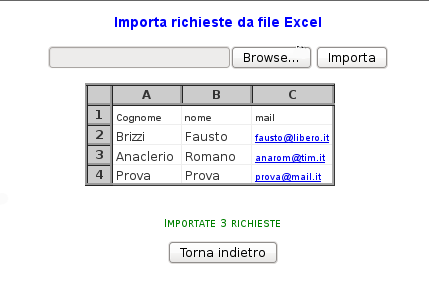
\includegraphics[scale=0.8]{./images/importaExcelScreen.png}
\caption{Importazione da file excel}
\label{excel}
\end{figure}

\noindent
Proprio grazie a questa possibilit\`a, la scansione riga per riga dei campi del foglio di calcolo (forniti appositamente con i dati voluti, in genere nome, cognome ed indirizzo e-mail), permette di inserire una richiesta di seguito all'altra, fino alla fine del file. L'amministratore potr\`a in seguito assegnare ai commerciali le richieste volute, oppure lasciarle nell'elenco pubblico. 
\newpage
La figura \ref{excel} mostra la fase terminale del processo, nella quale il sistema, richiamando tramite il controller la funzione \textit{leggi\_file}(), e utilizzando la libreria \textit{upload} di CodeIgniter per l'upload dei file.

\begin{figure}[!ht]
\centering
  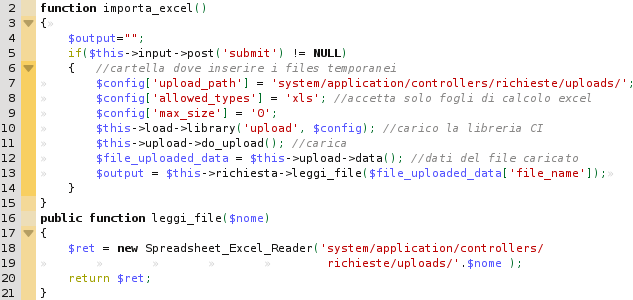
\includegraphics[scale=0.8]{./images/codiceexcel.png}
\caption{Codice PHP per la lettura di un file .xls}
\label{excelcode}
\end{figure}

\noindent
Per quanto riguarda invece la scansione della casella mail, serve una premessa: Tecnobit \`e affiliata a Bricsys\textregistered, societ\`a canadese sviluppatrice di Bricscad, il software pi\`u importante trattato dall'azienda, tradotto e venduto su suolo italiano. Si tratta di una soluzione alternativa e notevolmente pi\`u economica di Autocad\textregistered, soluzione leader del settore CAD di Autodesk Inc., compatibilile con il formato AutoCAD DWG utilizzato da quest'ultimo. Grazie a questa affiliazione, nel caso un cliente italiano scarichi la versione dimostrativa dal sito di Bricsys\textregistered, questa invia un mail standard a Tecnobit con i dati di questo cliente, in modo da permettere il contatto di questo cliente interessato all'acquisto del software in questione.
Per garantire quindi la possibilit\`a di aggiungere queste richieste al database, \`e stata usata la libreria \textit{\hyperlink{imap}{\underline{IMAP}}, POP3 e NNTP} di estensione al PHP \cite{quattro}, utile per leggere la casella di posta.
\newpage

\begin{figure}[!ht]
\centering
  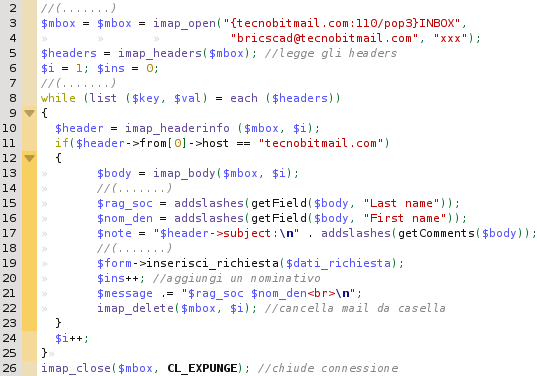
\includegraphics[scale=0.8]{./images/codicebrics.png}
\caption{Codice PHP per la lettura scansione della casella di posta}
\label{bricscode}
\end{figure}

\noindent La figura \ref{bricscode} illustra, con le dovute abbreviazioni, i passaggi relativi a questa operazione, richiamati dal controller tramite la funzione \textit{import\_bricscad}(), che iniziano con l'apertura della sessione IMAP e la lettura dei vari headers. Per ogni e-mail scansionata (che segue un template inviato dalla stessa Bricsys che mantiene tutti i campi inalterati) ne viene letto il contenuto, fino ad aggiungere una nuova richiesta con i dati raccolti tramite il solito metodo \textit{inserisci\_richiesta}(). Al termine della lettura, le mail lette vengono cancellate dalla casella di posta per evitare ripetizioni future.
Questa importazione \`e ovviamente consentita solo agli amministratori della sezione, che possono gestire come nel caso precedente le richieste importate, che tengono traccia comunque della fonte di provenienza, permettendo sempre di capire da dove sono state raccolte.

\newpage
\subsection{Test}
Per verificare che il componente sviluppato soddisfacesse correttamente tutte le funzionalit\`a l'azienda non richiedeva l'esecuzione di test di unit\`a costruiti appositamente o l'impiego di metodi di verifica e validazione, conscia anche del fatto che senza dei veri dati su cui lavorare (che saranno pronti una volta sviluppata la prevista migrazione) la maggior parte del codice non era testabile a fondo. In ogni caso le parti sono state utilizzate come prova dai dipendenti dell'azienda interessati, e in particolare con svariati esempi di importazione di alcuni file excel e la lettura con successo della casella e-mail, e numerosi tentativi di download dei dimostrativi dei programmi, testando ogni possibile prodotto in modo da verificare eventuali problemi. 
L'unica parte immediatamente (anche se non completamente) utilizzabile \`e stata quella riguardante i fax, in quanto i file di testo erano immediatamente disponibili all'uso, e quindi leggibili dai report sviluppati. 
Gli esempi sono stati provati usando i browser principali disponibili al momento: Internet Explorer, Firefox, Chrome, Safari ed Opera (tutti nelle ultime versioni disponibili, tranne Internet Explorer che \`e stato provato sia sulla versione 8 che sulla versione 7): la semplicit\`a del layout non ha portato a nessun problema grafico rilevante. Inoltre le views caricate da Voispeed tramite il suo visualizzatore, istanza di IE, sono state testate a fondo proprio con quest'ultimo.

\chapter{Problemi incontrati}
A proposito del modulo VoIP e Fax, il problema principale \`e stato di trovare un modo efficiente per gestire l'evento di chiusura di una chiamata, lasciando l'operatore sulla stessa pagina nel caso dell'inoltro di una telefonata, in quanto ogni volta che si rendeva necessario un inoltro, Voispeed interpretava la chiusura della chiamata con l'interno selezionato e  l'evento CALL\_CLOSE aggiornava la pagina del visualizzatore perdendo tutti i dati del cliente chiamante. \\
Per ovviare a questo problema si \`e deciso di gestire manualmente l'evento di chiusura della chiamata escludendolo dal controllo del client, in modo da far si che sia l'utente ad avere il pieno controllo della terminazione della telefonata. In tale modo un utente deve sempre chiudere manualmente la chiamata per far si che il sistema elabori correttamente le informazioni.\\
Nel caso dei fax ricevuti, si poneva invece il problema delle prestazioni. Infatti la lettura necessitava della scansione di tutte le righe una per una, come per i fax in arrivo, ma filtrati per utente, il che inizialmente rendeva i tempi di attesa (anche per ottenere solo un paio di fax nell'elenco) troppo elevati: per ovviare a questo problema, si \`e scelto di ottenere l'elenco dei fax associati a un singolo utente salvandoli in un array, per poi confrontarli con l'identificativo di ogni riga del file: in questo modo le prestazioni aumentavano visibilmente, rendendo finalmente fruibile il report. \\
Per quanto riguarda il modulo delle richieste, la difficolt\`a principale \`e stato il ragionamento basato su considerazioni molto teoriche (in quanto il regolamento commerciale interno, che regola il comportamento degli operatori nel loro lavoro e pone alcune limitazioni, \`e tuttora in fase di concepimento), che sicuramente andranno a modificare alcuni dettagli in futuro, soprattutto per quanto riguarda l'acquisizione delle richieste e la durata dei periodi di tutela su un cliente.

\chapter{Conclusioni}
\section{Risultati ottenuti durante lo stage}
Lo stage si \`e concluso positivamente: il lavoro assegnato \`e stato portato a termine completamente e nei tempi prestabiliti, rispettando il piano di lavoro preventivato, con qualche cambiamento nella distribuzione delle ore in particolare per la fase di codifica, e tutti i requisiti individuati in fase di analisi sono stati soddisfatti pienamente. 
I moduli sviluppati sono ultimati, ma per ora non ancora utilizzabili in quanto \`e strettamente necessaria la migrazione dal database vecchio al nuovo, in modo da poter lavorare su dati freschi ed aggiornati. \\
A seguito di una breve dimostrazione dell'operato svolto, anche con il lavoro di altri stagisti, l'azienda ha deciso di procedere con una integrazione parziale delle componenti al seguito di questa imminente migrazione. Questo permetter\`a di usufruire delle nuove parti sviluppate in sostituzione delle vecchie, in parallelo con il resto del sistema informativo, probabilmente effettuando una sincronizzazione continua dei dati, in modo che ognuno dei due database sia mantenuto aggiornato nel tempo, in attesa della completa adozione del nuovo sistema. \\
Alcuni possibili miglioramenti del prodotto potrebbero riguardare la creazione di nuovi filtri negli elenchi, sia dei fax che delle richieste, in modo da garantire una maggiore scrematura dei risultati, anche se nell'immediato tale bisogno non si pone.

\section{Conoscenze utilizzate ed acquisite}
Dal punto di vista tecnico all'inizio dello stage conoscevo la maggior parte delle tecnologie usate. Le nozioni che possedevo e si sono dimostrate essere sufficienti riguardavano l'\hyperlink{sql}{\underline{SQL}} e  le tecnologie per il Web come l'HTML e i CSS.. La parte in cui ho riscontrato maggiori difficolt\`a \`e stata quella inerente CodeIgniter e PHP. 
PHP \`e stata ovviamente la base di partenza, per poter poi comprendere il funzionamento del framework. La documentazione presente su \textit{php.net} \cite{quattro} \`e risultata ottima, con ogni metodo o costrutto discusso approfonditamente anche con esempi dell'utenza, che sono sempre di grossa utilit\`a in questi casi. \\
Per CodeIgniter ho trovato la documentazione ufficiale molto esauriente e semplice da comprendere, e mi sono inoltre rivolto a tutorials presenti in rete abbastanza completi. L'utilizzo del pattern MVC nella programmazione \`e stato un po' spiazzante inizialmente, in quanto necessitava di un approccio molto strutturato a monte, ma incredibilmente valido una volta abituaticisi. \\
Le funzioni di aiuto fornite da CodeIgniter hanno permesso di effettuare operazioni anche complesse in modo molto rapido, permettendo un risparmio di tempo non indifferente. Inoltre questa modalit\`a di sviluppo \`e stata molto proficua dal punto di vista didattico, in quanto l'interfacciamento di un'applicazione basata sul web con un DBMS \`e una materia di notevole interesse, anche in prospettiva lavorativa, e durante i corsi frequentati nessun progetto era arrivato ad integrare insieme tali tecnologie, trattandole sempre in sedi staccate tra loro. 

\section{Considerazioni personali}
Partendo dal presupposto che una delle motivazioni principali per la scelta di questo stage \`e stata appunto la curiosit\`a verso le tecnologie utilizzate, le competenze acquisite si possono definire soddisfacenti, sia in campo teorico che in campo pratico. Il lato pratico, oltre a far emergere problemi prima ignorati, fornisce anche una certa sicurezza nelle proprie conoscenze, necessaria ad effettuare le scelte richieste in fase di progettazione. Oltre alle conoscenze tecniche appena descritte, l'attivit\`a di stage permette anche di entrare in contatto con il mondo del lavoro. Quest'esperienza di quasi tre mesi \`e stata l'ideale per entrare nell'ottica aziendale. Rispetto ai progetti svolti durante i corsi universitari, infatti, i requisti sono molto meno definiti e i tempi per completare il prodotto sono estremamente ridotti. Questa ha portato anche ad intuire che nelle aziende locali la disciplina dell'ingegneria del software non abbia fatto particolarmente presa, in quanto si \`e potuto assistere a scelte che miravano pi\`u ad ottenere un prodotto apparentemente funzionante e commerciabile (\"{}dottrina\"{} seguita anche per lo sviluppo nel tempo del vecchio sistema informativo aziendale), piuttosto che ad un prodotto affidabile, frutto di processi produttivi di qualit\`a verificabile e migliorabile nel tempo.

\clearpage{\pagestyle{empty}\cleardoublepage
\addcontentsline{toc}{chapter}{Glossario}
\chapter*{Glossario}
\section*{C}
\hypertarget{css}{}
\textbf{CSS:}
CSS (Acronimo per Cascading Style Sheets) \`e un linguaggio utilizzato per descrivere la parte di presentazione di un documento scritto con un linguaggio di markup come HTML e XML. \\

\section*{D}
\hypertarget{dbms}{}
\textbf{DBMS:}
Un DBMS \`e un sistema software progettato per consentire la creazione e manipolazione efficiente di database (ovvero di collezioni di dati strutturati), solitamente da parte di pi\`u utenti.

\section*{F}
\hypertarget{framework}{}
\textbf{Framework:}
Un framework \`e una struttura di supporto su cui un software pu\`o essere organizzato e progettato con alla base sempre una serie di librerie di codice utilizzabili con uno o pi\`u linguaggi di programmazione, spesso fornite di una serie di strumenti di supporto allo sviluppo del software, come ad esempio un IDE, un debugger, o altri strumenti ideati per aumentare la velocit\`a di sviluppo del prodotto finito.

\section*{H}
\hypertarget{html}{}
\textbf{HTML:}
HTML \` e un linguaggio usato per descrivere la struttura dei documenti ipertestuali disponibili nel world wide web.
L'HTML non \` e un linguaggio di programmazione, ma un linguaggio di markup, ossia descrive il contenuto, testuale e non, di una pagina web.\\

\section*{I}
\hypertarget{imap}{}
\textbf{IMAP:}
L'IMAP (Internet Message Access Protocol) \`e un protocollo di comunicazione per la ricezione di e-mail, con alcune peculiarit\`a aggiuntive rispetto al \hyperlink{pop}{\underline{POP}} come l'accesso alla posta sia online che off-line, utenza multipla e il supporto all'accesso a singole parti di un messaggio.

\section*{J}
\hypertarget{javascript}{}
\textbf{JavaScript:}
JavaScript (o ECMAScript) \`e un linguaggio di scripting orientato agli oggetti comunemente usato nei siti web. \`E  uno standard ISO.\\

\section*{L}
\hypertarget{lamp}{}
\textbf{LAMP:}
LAMP \`e un acronimo che indica una piattaforma per lo sviluppo di applicazioni web che prende il nome dalle iniziali dei componenti software con cui è realizzata, ossia GNU/\textbf{L}inux: il sistema operativo; \textbf{A}pache: il Web server; \textbf{M}ySQL: il database management system (o database server); \textbf{P}erl, \textbf{P}HP e/o \textbf{P}ython: i linguaggi di scripting.

\section*{M}
\hypertarget{mail_server}{}
\textbf{Mail Server:}
Un mail server (Mail Transfer Agent o MTA) \`e un programma, e per estensione il computer su cui viene eseguito, che si occupa dello smistamento da un computer a un altro della posta elettronica.\\

\section*{O}
\hypertarget{opensource}{}
\textbf{Open Source:}
Con il termine Open Source si indica un tipo di licenza software in cui il codice sorgente viene reso disponibile; lo scopo dell'Open Source \`e quello di favorire la collaborazione tra gli sviluppatori e il progresso del software tramite la condivisione di idee.\\

\section*{P}
\hypertarget{pop}{}
\textbf{POP:}
Il POP (Post Office Protocol) \`e un protocollo che ha il compito di permettere, mediante autenticazione, l'accesso ad un account di posta elettronica presente su di un host per scaricare le e-mail del relativo account.\\

\section*{R}
\hypertarget{report}{}
\textbf{Report:}
Un report \`e un documento generalmente costituito da visualizzazioni tabellari e grafiche di parti ritenute particolarmente importanti per l'utilizzatore.

\section*{S}
\hypertarget{server}{}
\textbf{Server:}
Il server \`e una componente informatica software o hardware che fornisce servizi ad altre componenti chiamate client attraverso una rete. \\


\hypertarget{sql}{}
\noindent
\textbf{SQL:}
SQL (Structured Query Language) \`e un linguaggio di programmazione per database progettato per leggere, modificare e gestire dati memorizzati in un sistema basato sul modello relazionale, per creare e modificare schemi di database e per creare e gestire strumenti di controllo ed accesso ai dati.\\

\section*{U}
\hypertarget{uml}{}
\textbf{UML:}
UML (Unified Modeling Language) \`e un  linguaggio di modellazione e specica basato sul paradigma object-oriented che consente di descrivere in modo standard ed efficace sistemi complessi.\\

\hypertarget{url}{}
\noindent 
\textbf{URL:}
Un URL (Uniform Resource Locator) \`e una sequenza di caratteri dal formato standard che identifica univocamente l'indirizzo di una risorsa sulla rete Internet.

\section*{W}
\hypertarget{w3c}{}
\textbf{W3C:}
W3C, abbreviazione di World Wide Web Consortium, \`e un'associazione nata con lo scopo di migliorare gli esistenti protocolli e linguaggi per il Web, facilitandone lo sviluppo, la diffusione ed il potenziamento.

\clearpage{\pagestyle{empty}\cleardoublepage


\begin{thebibliography}{9}
\addcontentsline{toc}{chapter}{Bibliografia}
\bibitem{uno} Guida in linea di CodeIgniter\\ \url{http://codeigniter.com/user\_guide/}
\bibitem{cistyle} Guida allo stile di codifica di CodeIgniter\\ \url{http://codeigniter.com/user_guide/general/styleguide.html}
\bibitem{due} W3C\\ \url{http://www.w3.org/}
\bibitem{tre} Wikipedia\\ \url{http://www.wikipedia.org}
\bibitem{quattro} PHP Official Documentation\\ \url{http://www.php.net/docs.php}
\bibitem{excel reader} PHP Excel Reader Homepage \\\url{http://code.google.com/p/php-excel-reader}
\bibitem{cinque} PHP Excel Reader Documentation\\ \url{http://code.google.com/p/php-excel-reader/wiki/Documentation}
\bibitem{jquery} jQuery Official Documentation\\ \url{http://docs.jquery.com/Main_Page}
\bibitem{voispeed} Manuale Voispeed PLATFORM \\ \url{http://www.voispeed.com/man/platform/it/44/manuale.htm}
\end{thebibliography}
\end{document}